\pdfinfoomitdate=1
\pdftrailerid{}
\pdfsuppressptexinfo=-1
\documentclass[10pt,a4paper]{article}
\usepackage{cmap}
\usepackage[margin=1.8cm,headheight=14pt,headsep=10pt]{geometry}
\usepackage[leqno]{amsmath}
\usepackage{amssymb,booktabs,longtable,array,ragged2e,multicol,multirow,xcolor,fancyhdr,tikz}
\definecolor{linkblue}{rgb}{0.08,0.33,0.58}
\usepackage[colorlinks=true,linkcolor=linkblue,urlcolor=linkblue,citecolor=linkblue,
  filecolor=linkblue,linktoc=all,pdfborder={0 0 0},bookmarksnumbered=true]{hyperref}
\setlength{\parindent}{0pt}\setlength{\parskip}{4pt}
\setcounter{secnumdepth}{2}\setcounter{tocdepth}{2}
\definecolor{partshade}{gray}{0.9}
\usepackage{nicefrac}
\definecolor{parttitle}{HTML}{295A2C}
\definecolor{parttitlelight}{HTML}{6C9F6D}
\makeatletter
\renewcommand\section{\@startsection{section}{1}{\z@}{-3ex plus -1ex minus -.2ex}%
  {1.2ex plus .2ex}{\normalfont\large\sffamily\bfseries\color{parttitle}}}
\renewcommand\subsection{\@startsection{subsection}{2}{\z@}{-2.5ex plus -1ex minus -.2ex}%
  {.8ex plus .2ex}{\normalfont\sffamily\bfseries\color{parttitle}}}
\renewcommand\subsubsection{\@startsection{subsubsection}{3}{\z@}{-2ex plus -1ex minus -.2ex}%
  {.6ex plus .2ex}{\normalfont\small\sffamily\bfseries\color{parttitle}}}
\renewcommand\paragraph{\@startsection{paragraph}{4}{\z@}{1.5ex plus .5ex minus .2ex}{-1em}%
  {\normalfont\small\sffamily\bfseries\color{parttitle}}}
\renewcommand\tagform@[1]{\maketag@@@{\textsf{\bfseries\footnotesize (#1)}}}
\renewcommand*\l@part[2]{\par\addvspace{1.6ex}\noindent{\sffamily\bfseries #1}\hfill
  {\sffamily\bfseries #2}\par\nobreak}
\newcommand\tocnumber{1.8em}
\newcommand\tocline[4]{\par{\rightskip \tocnumber plus 1fil\relax\parfillskip -\rightskip
  \noindent\hangindent\dimexpr#1+#2\relax\hspace*{#1}%
  \@tempdima #2{\sffamily\small #3}\nobreak\leaders\hbox{$\m@th\mkern 4.5mu\hbox{.}%
  \mkern 4.5mu$}\hfill\nobreak\hbox to \tocnumber{\hfil\sffamily\small #4}\par}}
\renewcommand*\l@section[2]{\tocline{0em}{2.2em}{#1}{#2}}
\renewcommand*\l@subsection[2]{\tocline{2.2em}{2.6em}{#1}{#2}}
\newcommand\contentspage{{\setlength{\columnsep}{24pt}\begin{multicols}{2}\@starttoc{toc}%
  \end{multicols}}}
\newcounter{docpart}\@addtoreset{section}{docpart}
\renewcommand\thesection{\ifnum\value{docpart}>0 \arabic{docpart}.\fi\arabic{section}}
\renewcommand\theHsection{\arabic{docpart}.\arabic{section}}
\newcommand\partnumber[1]{#1\enspace}
\pdfstringdefDisableCommands{\def\partnumber#1{#1 }}
\newcommand{\partbox}[1]{\par\addvspace{12pt}\refstepcounter{docpart}\phantomsection
  \addcontentsline{toc}{part}{\protect\partnumber{\thedocpart}#1}%
  \noindent\colorbox{partshade}{\makebox[%
  \dimexpr\textwidth-2\fboxsep\relax]{\rule[-6pt]{0pt}{20pt}\Large\sffamily\bfseries%
  \textcolor{parttitle}{\thedocpart\quad #1}}}\par\nobreak\@nobreaktrue\addvspace{2pt}}
\newmarks\LTstartmarks\newcount\LTstartcount
\let\LT@startplain\LT@start
\def\LT@start{\global\advance\LTstartcount\@ne\LT@startplain
  \marks\LTstartmarks{\the\LTstartcount}}
\newmarks\LTgroupmarks
\newcount\LTspacebreak\LTspacebreak=-1
\newcount\LTrulebreak\LTrulebreak=-2
\def\grouprule#1#2{\noalign{\marks\LTgroupmarks{\the\belowrulesep}\nobreak\vskip#1%
  \vskip\aboverulesep}\multispan\LT@cols\unskip{\leaders\hrule\@height#2\hfill\kern\z@}\cr
  \noalign{\penalty\LTrulebreak\vskip\belowrulesep\global\@lastruleclass\z@}}
\def\groupspace#1{\noalign{\marks\LTgroupmarks{\the\dimexpr#1\relax}\penalty\LTspacebreak
  \vskip#1\global\@lastruleclass\z@}}
\def\LT@unskips{\unskip\unpenalty\unskip\unpenalty\unskip\unpenalty\unskip\unpenalty}
\def\LT@groupcut{\ifnum\outputpenalty=\LTrulebreak
  \setbox\@cclv\vbox{\unvbox\@cclv\setbox\z@\lastbox\LT@unskips}\fi}
\def\LT@groupjoin{\ifnum\outputpenalty=\LTspacebreak\vskip-\botmarks\LTgroupmarks\relax\fi
  \ifnum\outputpenalty=\LTrulebreak\vskip-\botmarks\LTgroupmarks\relax\fi}
\let\LT@outputplain\LT@output
\def\LT@output{\ifnum\outputpenalty<-\@Mi\LT@outputplain\else
  \edef\LT@marka{\botmarks\LTstartmarks}\edef\LT@markb{\the\LTstartcount}%
  \ifx\LT@marka\LT@markb\LT@groupcut\LT@outputplain\LT@groupjoin
  \else\setbox\LT@head\box\voidb@x\LT@outputplain\fi\fi}
\makeatother
\newcommand{\needspace}[1]{\par\penalty-100\begingroup\dimen0=#1\relax\dimen2=\pagegoal
  \advance\dimen2-\pagetotal\ifdim\dimen0>\dimen2\relax\ifdim\dimen2>0pt\vfil\break\fi\fi
  \endgroup}
\numberwithin{equation}{section}
\pagestyle{fancy}\fancyhf{}
\renewcommand{\headrulewidth}{0pt}
\renewcommand{\sectionmark}[1]{\markright{\thesection\enspace #1}}
\renewcommand{\subsectionmark}[1]{}
\fancyhead[R]{\small\textsc{\rightmark}\quad\thepage}
\fancypagestyle{plain}{\fancyhf{}\fancyfoot[C]{\small\thepage}}
\definecolor{atlasI}{HTML}{991A1A}\definecolor{atlasIl}{HTML}{EC6B60}
\definecolor{atlasII}{HTML}{295A2C}\definecolor{atlasIIl}{HTML}{6C9F6D}
\definecolor{atlasIII}{HTML}{7A1466}\definecolor{atlasIIIl}{HTML}{D66EBC}
\definecolor{atlasIV}{HTML}{9B690B}\definecolor{atlasIVl}{HTML}{F2A618}
\makeatletter
\newcommand\atlas@full{%
\fill[atlasIII] (0.0394,0.0163) -- (0.3978,0.0163) arc[start angle=0.668, end angle=13.836, radius=1.3979] -- cycle;
\fill[atlasI] (-0.0163,0.0394) -- (-0.0163,0.3978) arc[start angle=90.668, end angle=103.836, radius=1.3979] -- cycle;
\fill[atlasIV] (-0.0394,-0.0163) -- (-0.3978,-0.0163) arc[start angle=-179.332, end angle=-166.164, radius=1.3979] -- cycle;
\fill[atlasII] (0.0163,-0.0394) -- (0.0163,-0.3978) arc[start angle=-89.332, end angle=-76.164, radius=1.3979] -- cycle;
\fill[atlasIIIl] (0.0163,0.0394) -- (0.3343,0.3573) arc[start angle=76.164, end angle=89.332, radius=1.3979] -- cycle;
\fill[atlasIl] (-0.0394,0.0163) -- (-0.3573,0.3343) arc[start angle=166.164, end angle=179.332, radius=1.3979] -- cycle;
\fill[atlasIVl] (-0.0163,-0.0394) -- (-0.3343,-0.3573) arc[start angle=-103.836, end angle=-90.668, radius=1.3979] -- cycle;
\fill[atlasIIl] (0.0394,-0.0163) -- (0.3573,-0.3343) arc[start angle=-13.836, end angle=-0.668, radius=1.3979] -- cycle;
\fill[atlasIIIl] (0.4304,0.0163) -- (0.9598,0.0163) arc[start angle=46.637, end angle=73.849, radius=1.3979] arc[start angle=13.862, end angle=0.653, radius=1.4305] -- cycle;
\fill[atlasIl] (-0.0163,0.4304) -- (-0.0163,0.9598) arc[start angle=136.637, end angle=163.849, radius=1.3979] arc[start angle=103.862, end angle=90.653, radius=1.4305] -- cycle;
\fill[atlasIVl] (-0.4304,-0.0163) -- (-0.9598,-0.0163) arc[start angle=-133.363, end angle=-106.151, radius=1.3979] arc[start angle=-166.138, end angle=-179.347, radius=1.4305] -- cycle;
\fill[atlasIIl] (0.0163,-0.4304) -- (0.0163,-0.9598) arc[start angle=-43.363, end angle=-16.151, radius=1.3979] arc[start angle=-76.138, end angle=-89.347, radius=1.4305] -- cycle;
\fill[atlasIII] (0.0163,0.4304) arc[start angle=89.347, end angle=76.138, radius=1.4305] arc[start angle=16.151, end angle=43.363, radius=1.3979] -- cycle;
\fill[atlasI] (-0.4304,0.0163) arc[start angle=179.347, end angle=166.138, radius=1.4305] arc[start angle=106.151, end angle=133.363, radius=1.3979] -- cycle;
\fill[atlasIV] (-0.0163,-0.4304) arc[start angle=-90.653, end angle=-103.862, radius=1.4305] arc[start angle=-163.849, end angle=-136.637, radius=1.3979] -- cycle;
\fill[atlasII] (0.4304,-0.0163) arc[start angle=-0.653, end angle=-13.862, radius=1.4305] arc[start angle=-73.849, end angle=-46.637, radius=1.3979] -- cycle;
\fill[atlasIII] (0.9997,0.0232) arc[start angle=1.329, end angle=44.066, radius=1] -- (0.3973,0.3742) arc[start angle=73.875, end angle=45.664, radius=1.4305] -- cycle;
\fill[atlasI] (-0.0232,0.9997) arc[start angle=91.329, end angle=134.066, radius=1] -- (-0.3742,0.3973) arc[start angle=163.875, end angle=135.664, radius=1.4305] -- cycle;
\fill[atlasIV] (-0.9997,-0.0232) arc[start angle=-178.671, end angle=-135.934, radius=1] -- (-0.3973,-0.3742) arc[start angle=-106.125, end angle=-134.336, radius=1.4305] -- cycle;
\fill[atlasII] (0.0232,-0.9997) arc[start angle=-88.671, end angle=-45.934, radius=1] -- (0.3742,-0.3973) arc[start angle=-16.125, end angle=-44.336, radius=1.4305] -- cycle;
\fill[atlasIIIl] (0.0232,0.9997) arc[start angle=44.336, end angle=16.125, radius=1.4305] -- (0.6955,0.7185) arc[start angle=45.934, end angle=88.671, radius=1] -- cycle;
\fill[atlasIl] (-0.9997,0.0232) arc[start angle=134.336, end angle=106.125, radius=1.4305] -- (-0.7185,0.6955) arc[start angle=135.934, end angle=178.671, radius=1] -- cycle;
\fill[atlasIVl] (-0.0232,-0.9997) arc[start angle=-135.664, end angle=-163.875, radius=1.4305] -- (-0.6955,-0.7185) arc[start angle=-134.066, end angle=-91.329, radius=1] -- cycle;
\fill[atlasIIl] (0.9997,-0.0232) arc[start angle=-45.664, end angle=-73.875, radius=1.4305] -- (0.7185,-0.6955) arc[start angle=-44.066, end angle=-1.329, radius=1] -- cycle;
}
\newcommand\atlas@draw[2]{\begin{tikzpicture}[x=\dimexpr(#1)/2\relax,y=\dimexpr(#1)/2\relax]
\useasboundingbox (-1,-1) rectangle (1,1);#2\end{tikzpicture}}
\newcommand\atlas@volume[1]{{%
\colorlet{atlasI}{parttitle}\colorlet{atlasIl}{parttitlelight}%
\colorlet{atlasII}{parttitle}\colorlet{atlasIIl}{parttitlelight}%
\colorlet{atlasIII}{parttitle}\colorlet{atlasIIIl}{parttitlelight}%
\colorlet{atlasIV}{parttitle}\colorlet{atlasIVl}{parttitlelight}%
#1}}
\newcommand\atlasmark[1]{\atlas@draw{#1}{\atlas@full}}
\newcommand\volumemark[1]{\atlas@volume{\atlasmark{#1}}}
\makeatother
\fancypagestyle{opening}{\fancyhf{}\fancyfoot[C]{\small\thepage}%
  \fancyhead[L]{\smash{\raisebox{-9.5mm}{\volumemark{12mm}}}}}
\hypersetup{pdftitle={2C6: Point Group Atlas, volume II: double point groups}, pdfsubject={Point Group Atlas double record 2C6, schema point-group-atlas/double/group/1}}
\fancyhead[L]{\small $\grp{2C_{6}}$}
\DeclareMathAlphabet{\mathelt}{OT1}{cmss}{m}{sl}
\DeclareSymbolFont{eltgreek}{OML}{cmssm}{m}{it}
\DeclareMathSymbol{\eltsigma}{\mathord}{eltgreek}{"1B}
\DeclareSymbolFont{eltletters}{OT1}{cmss}{m}{sl}
\DeclareMathSymbol{g}{\mathalpha}{eltletters}{`g}
\DeclareMathSymbol{h}{\mathalpha}{eltletters}{`h}
\DeclareMathSymbol{Q}{\mathalpha}{eltletters}{`Q}
\DeclareMathSymbol{R}{\mathalpha}{eltletters}{`R}
\DeclareMathSymbol{\xi}{\mathord}{eltgreek}{"18}
\newcommand{\eltfont}[1]{{\let\sigma\eltsigma\mathelt{#1}}}
\newcommand{\grp}[1]{\mathsf{#1}}
\newcommand{\irr}[1]{\text{\normalfont\scshape #1}}
\newcommand{\conjpair}[1]{{}^{#1}}
\newcommand{\detbox}[1]{{\setlength{\fboxsep}{1pt}\fbox{#1}}}
\newcommand{\cls}[1]{\eltfont{#1}}
\newcommand{\comp}[1]{\eltfont{#1}}
\newcommand{\elt}[1]{\eltfont{#1}}
\newcommand{\hmname}[1]{#1}
\newcommand{\conwayname}[1]{#1}
\newcommand{\ptag}[1]{\mathrm{#1}}
\newcommand{\orbital}[1]{\mathrm{#1}}
\newcommand{\dirprod}{\times}
\newcommand{\sdprod}{\rtimes}
\newcommand{\samecls}{\cong}
\newcommand{\nconj}[1]{{\scriptsize$\times#1$}}
\newcommand{\clsletter}[1]{\,{\scriptsize\color{black!55}#1}}
\newcommand{\metclasses}[1]{\,{\scriptsize$\{#1\}$}}
\newcommand{\Cyc}[1]{\grp{Z_{#1}}}
\newcommand{\Sym}[1]{\grp{Sym_{#1}}}
\newcommand{\dirvec}[3]{(#1, #2, #3)}
\newcommand{\grpindex}[2]{[#1 : #2]}
\newcommand{\iverson}[1]{[#1]}
\newcommand{\restr}[2]{#1\!\downarrow#2}
\newcommand{\Ind}[2]{\operatorname{Ind}_{#1}^{#2}}
\newcommand{\genidx}[2]{#1^{[\mathrm{#2}]}}
\newcommand{\pointr}{\mathbf{r}}
\newcommand{\unitaxis}{\hat{\mathbf{v}}}
\newcommand{\vv}{\mathbf{v}}
\newcommand{\iunit}{\mathrm{i}}
\newcommand{\expe}{\mathrm{e}}
\newcommand{\diff}{\mathrm{d}}
\newcommand{\goldenratio}{\varphi}
\newcommand{\rootunity}[1]{\zeta_{#1}}
\newcommand{\irrJ}[1]{D^{(#1)}}
\newcommand{\irrJp}[2]{D^{(#1,#2)}}
\newcommand{\repD}[1]{D^{#1}}
\newcommand{\wignerD}[1]{D^{#1}}
\newcommand{\wignerd}[1]{d^{#1}}
\newcommand{\irchar}[1]{\chi_{#1}}
\newcommand{\chiA}{\chi_{\grp{A}}}
\newcommand{\fsind}{\nu_{\mathrm{FS}}}
\newcommand{\conj}[1]{{#1}^{*}}
\newcommand{\diag}{\operatorname{diag}}
\newcommand{\trace}{\operatorname{tr}}
\newcommand{\irrprod}{\otimes}
\newcommand{\mult}{\kappa}
\newcommand{\intx}{\mu}
\newcommand{\cgnorm}{\mathcal{N}}
\newcommand{\period}{L}
\newcommand{\jm}[2]{\bigl\lvert{}^{#1}_{\,#2}\bigr\rangle}
\newcommand{\cgket}[3]{\bigl\lvert{}^{#1}_{\,#2};#3\bigr\rangle}
\newcommand{\irket}[2]{\bigl\lvert{}^{#1}_{\,#2}\bigr\rangle}
\newcommand{\prodket}[2]{\lvert {#1}\,{#2}\rangle}
\newcommand{\ket}[1]{\lvert #1\rangle}
\newcommand{\cgc}[6]{\bigl\langle{}^{#1}_{\,#2}\,{}^{#3}_{\,#4}\bigm\vert{}^{#5}_{\,#6}\bigr\rangle}
\newcommand{\cgck}[7]{\bigl\langle{}^{#1}_{\,#2}\,{}^{#3}_{\,#4}\bigm\vert{}^{#5}_{\,#6};#7\bigr\rangle}
\newcommand{\cgcone}[3]{\langle #1\,#2\mid #3\rangle}
\newcommand{\irrangle}{\text{--}}
\newcommand{\vol}{\operatorname{vol}}
\newcommand{\fcell}{\mathcal{D}}
\newcommand{\fdomain}{\mathcal{F}}
\newcommand{\lensspace}[2]{\mathsf{L}(#1, #2)}
\newcommand{\twosphere}{\mathsf{S}^{2}}
\newcommand{\projplane}{\mathbb{R}\mathsf{P}^{2}}
\newcommand{\term}[2]{{}^{#1}#2}
\newcommand{\barred}[1]{\bar{#1}}
\newcommand{\Quat}[1]{\grp{Q_{#1}}}
\newcommand{\SL}[1]{\grp{SL}(2,#1)}
\newcommand{\secondclass}{\mathrm{b}}
\newcommand{\dmark}{{}^{d}}
\newcommand{\lift}[1]{\tilde{#1}}
\newcommand{\pauli}[1]{\sigma_{#1}}
\newcommand{\paulivec}{\vec{\sigma}}
\newcommand{\hairsp}{\mkern1mu}
\newenvironment{romanlist}{\begin{enumerate}%
\renewcommand{\labelenumi}{(\roman{enumi})}}%
  {\end{enumerate}}
\makeatletter
\newenvironment{irmatrix}[1]{\null\,\vcenter\bgroup\Let@\restore@math@cr\default@tag
  \baselineskip8\ex@ \lineskip3\ex@ \lineskiplimit\lineskip
  \ialign\bgroup\hfil$\m@th\scriptstyle##$\hfil&&\hskip#1\hfil$\m@th\scriptstyle##$\hfil\crcr}%
  {\crcr\egroup\egroup\,}
\makeatother
\newlength{\fillwidth}\newlength{\cellwidth}\newlength{\colwidth}
\newcommand{\cellmax}[1]{\settowidth{\cellwidth}{#1}%
  \ifdim\cellwidth>\colwidth\setlength{\colwidth}{\cellwidth}\fi}
\newcommand{\fillcap}{\ifdim\colwidth<\fillwidth\setlength{\fillwidth}{\colwidth}\fi}
\newcommand{\signbreak}{\penalty100\relax}
\begin{document}
\thispagestyle{opening}
\begin{center}
{\LARGE\sffamily\bfseries\color{parttitle}The $\grp{2C_{6}}$ subgroup of $\grp{Pin^{-}(3)}$}
\end{center}
\contentspage
\needspace{194pt}
\partbox{The group}
\section{Names and structure}\label{s:identification}
Conventions: \href{../../CONVENTIONS.pdf}{CONVENTIONS.pdf}, sections \href{../../../rotation/CONVENTIONS.pdf\#conv.0.1}{0.1}, \href{../../../rotation/CONVENTIONS.pdf\#conv.2}{2}, \href{../../../rotation/CONVENTIONS.pdf\#conv.12}{12}, \href{../../CONVENTIONS.pdf\#conv.20}{20} and \href{../../CONVENTIONS.pdf\#conv.28}{28}.
{\small\begin{longtable}{@{}ll@{}}\toprule
\texttt{symbol} & \href{2C6.pdf}{$\grp{2C_{6}}$}\\
\texttt{cover\symbol{95}of} & \href{../../../rotation/data/pdf/C6.pdf}{$\grp{C_{6}}$}\\
\grouprule{0pt}{\lightrulewidth}
\texttt{abstract\symbol{95}type} & $\Cyc{12}$\\
\texttt{order} & 12\\
\texttt{gap\symbol{95}smallgroup\symbol{95}id} & [12, 2]\\
\grouprule{0pt}{\lightrulewidth}
\texttt{su2\symbol{95}subgroup} & \href{2C6.pdf}{$\grp{2C_{6}}$}, index 1\\
\texttt{normalizer} & \href{2Dinfh.pdf}{$\grp{2D_{\infty h}}$}\\
\texttt{centralizer} & \href{2Cinfh.pdf}{$\grp{2C_{\infty h}}$}, index 2 in the normalizer\\
\texttt{product\symbol{95}form} & \begin{tabular}[t]{@{}l@{}}direct: \href{2C2.pdf}{$\grp{2C_{2}}$}${}\dirprod{}$\href{C3.pdf}{$\grp{C_{3}}$}\end{tabular}\\
\texttt{center} & \href{2C6.pdf}{$\grp{2C_{6}}$}, index 1\\
\texttt{commutator\symbol{95}subgroup} & \href{C1.pdf}{$\grp{C_{1}}$}, index 12\\
\grouprule{0pt}{\lightrulewidth}
\texttt{altmann\symbol{95}T} & 6\\
\texttt{conway\symbol{95}smith} & $\conwayname{\grp{2C_{6}}}$\\
\texttt{hermann\symbol{95}mauguin} & $\dmark\hmname{6}$\\
\bottomrule\end{longtable}}
\leavevmode\label{n:element.inversion}\label{n:group.preimage}The group $\grp{2C_{6}}$ is the preimage in $\grp{Pin^{-}(3)}$ of \href{../../../rotation/data/pdf/C6.pdf}{$\grp{C_{6}}$}, whose document sets the fields that this table does not repeat (\texttt{cover\symbol{95}of}): its type, family, geometry, crystal classes and the names of its \href{../../../rotation/data/pdf/O3.pdf}{$\grp{O(3)}$}-conjugacy class. The field \texttt{su2\symbol{95}subgroup} is $\grp{2C_{6}} \cap \grp{SU(2)}$, the largest subgroup of $\grp{2C_{6}}$ in $\grp{SU(2)}$ (its elements of parity $+1$), and \texttt{normalizer} and \texttt{centralizer} are taken in $\grp{Pin^{-}(3)}$. The fields \texttt{center} and \texttt{commutator\symbol{95}subgroup} are classes of the table of section~\ref{s:subgroups}.
\needspace{103pt}
\section{The cover}\label{s:cover}
Conventions: \href{../../CONVENTIONS.pdf}{CONVENTIONS.pdf}, sections \href{../../CONVENTIONS.pdf\#conv.20.1}{20.1}, \href{../../CONVENTIONS.pdf\#conv.21.1}{21.1} and \href{../../CONVENTIONS.pdf\#conv.21.2}{21.2}.
\leavevmode\label{n:group.pin.minus}\label{n:group.su2}\label{n:local.pin.sign}\label{n:matrix.covered}\label{n:matrix.lift.su2}\label{n:index.bar}The point group $\grp{C_{6}}$ has the preimage $\grp{2C_{6}}$ in $\grp{Pin^{-}(3)} = \grp{SU(2)} \dirprod \{+1, -1\}$, whose element $(U, \varepsilon)$ covers $\varepsilon R(U) \in \grp{O(3)}$, where $U$ covers the rotation $R(U)$. The preimage is the double group of $\grp{C_{6}}$, with the $2 \cdot 6 = 12$ elements $(g, 0) = (U(g), \det g)$ and $(g, 1) = (-U(g), \det g)$, $g \in \grp{C_{6}}$, where $U(g)$ is the canonical lift of $g$ to $\grp{SU(2)}$ (\href{../../CONVENTIONS.pdf}{CONVENTIONS.pdf}, section \href{../../CONVENTIONS.pdf\#conv.21.1}{21.1}). \label{n:function.cocycle}With $U(h)\,U(g) = (-1)^{c(g,h)}\,U(gh)$, $gh$ = first $g$, then $h$, the product is
\begin{equation}\label{e:product}(g, b)(h, b') = \bigl(gh,\ b + b' + c(g, h) \bmod 2\bigr).\end{equation}
\leavevmode\label{n:mark.bar}The covering map $(g, b) \mapsto g$ has kernel $\{\elt{E}, \elt{\barred{E}}\}$, where $\elt{\barred{E}} = (\elt{E}, 1)$ is central of order 2. \label{n:element.named}\label{n:mark.lift}The barred partner $\elt{\barred{X}}$ of an element $\elt{X}$ of $\grp{C_{6}}$ is $(\elt{X}, 1)$, and the lift of the inversion, $\elt{\lift{i}} = (1, -1)$, is central of order 2.
\needspace{122pt}
\section{Symmetry operations}\label{s:elements}
Conventions: \href{../../CONVENTIONS.pdf}{CONVENTIONS.pdf}, sections \href{../../../rotation/CONVENTIONS.pdf\#conv.4}{4}, \href{../../../rotation/CONVENTIONS.pdf\#conv.5.1}{5.1} and \href{../../CONVENTIONS.pdf\#conv.21}{21}.
\leavevmode\label{n:index.element}\label{n:element.g}Element $k$ of $\grp{2C_{6}}$ is the pair $(g, b)$ of the element $g$ of \href{../../../rotation/data/pdf/C6.pdf}{$\grp{C_{6}}$} of index $\lfloor k/2\rfloor$ in its document and $b = k - 2\lfloor k/2\rfloor$. The pair $(g, 0)$ is the canonical lift of $g$, and $(g, 1)$ is its barred partner (section~\ref{s:cover}). \label{n:matrix.element.pin}\label{n:matrix.element}The matrix $M(k)$ of the element is the transpose of its $\grp{SU(2)}$ part $(-1)^{b}\,U(g)$, and the matrices compose as the matrices $P(g)$ of the elements of $\grp{C_{6}}$:
\begin{equation}\label{e:mprod}M(k)\,M(k') = M(kk'),\qquad kk' = \text{first } k\text{, then } k'.\end{equation}
\leavevmode\label{n:angle.omega}\label{n:vector.axis}\label{n:vector.pole}That part is the lift $\lift{R}_{\vv}(\omega)$, $0 \le \omega < 4\pi$, of the rotation part $(\det g)\,g$ of the element, about the axis $\vv$ of $g$ (a dash for none, \href{../../CONVENTIONS.pdf}{CONVENTIONS.pdf}, section \href{../../CONVENTIONS.pdf\#conv.21.1}{21.1}). \label{n:angle.euler.alpha}\label{n:angle.euler.beta}\label{n:angle.euler.gamma}\label{n:vector.coordinates}The Euler angles of the rotation part are $(\alpha,\beta,\gamma)$: by $\alpha$ about $z$, then by $\beta$ about $y$, then by $\gamma$ about $z$ (fixed axes). \label{n:local.euler.sign}The sign $s$ of the lift satisfies
\begin{equation}\label{e:euler}(-1)^{b}\,U(g) = s\,\expe^{-\iunit\gamma\pauli{z}/2}\,\expe^{-\iunit\beta\pauli{y}/2}\,\expe^{-\iunit\alpha\pauli{z}/2}.\end{equation}
\leavevmode\label{n:index.element.inverse}\label{n:head.sym}\label{n:head.ord}A row gives the index $k$ of the element, its symbol (sym, barred for a barred partner), its order (ord) and the index $k^{-1}$ of its inverse. \label{n:head.class}The class of the element is set with its size before its symbol (section~\ref{s:classes}).
The table lists the canonical lifts $(g, 0)$, of even $k$. The barred partner $(g, 1) = \elt{\barred{E}}\,(g, 0)$, of index $k + 1$, has the barred symbol and class, the same $\det$, $(\alpha,\beta,\gamma)$ and axis, $\omega + 2\pi$ modulo $4\pi$, the sign $-s$ and the matrix $-M(k)$. Its order and inverse (\texttt{elements.items}) are read from $\omega + 2\pi$ and the multiplication table.
\leavevmode\label{n:constant.root}\label{n:index.root.order}Exact values are rationals, square roots, cosines and sines of rational multiples of $\pi$, and the constants
\begin{equation}\label{e:constants}\rootunity{n} = \expe^{2\pi\iunit/n}\quad(n = 3, 12),\end{equation}
where $\iunit$ is the imaginary unit and $\expe$ is the base of the natural logarithm.
{\small\setlength{\tabcolsep}{4pt}
{\renewcommand{\arraystretch}{1.3}\begin{longtable}{@{}rlllrrlrlll@{}}\toprule
$k$ & sym & class & $\det$ & ord & $k^{-1}$ & $(\alpha,\beta,\gamma)$ & $s$ & $\omega$ & $\vv$ & $M(k)$\\\midrule\endhead
\bottomrule\endfoot\endlastfoot
0 & $\cls{E}$ & $\cls{E}$ & $+1$ & 1 & 0 & $(0,0,0)$ & $+1$ & $0$ & --- & $\left(\begin{irmatrix}{0.2778em}1 & 0\\0 & 1\end{irmatrix}\right)$\\*\addlinespace[6pt]
2 & $\cls{C_{6}}$ & $\cls{C_{6}}$ & $+1$ & 12 & 10 & $(0,0,\tfrac{\pi}{3})$ & $+1$ & $\tfrac{\pi}{3}$ & $\dirvec{0}{0}{1}$ & $\left(\begin{irmatrix}{0.2778em}-\rootunity{12}^{5} & 0\\0 & \rootunity{12}\end{irmatrix}\right)$\\\groupspace{6pt}
4 & $\cls{C_{3}}$ & $\cls{C_{3}}$ & $+1$ & 6 & 8 & $(0,0,\tfrac{2\pi}{3})$ & $+1$ & $\tfrac{2\pi}{3}$ & $\dirvec{0}{0}{1}$ & $\left(\begin{irmatrix}{0.2778em}-\rootunity{3} & 0\\0 & -\rootunity{3}^{2}\end{irmatrix}\right)$\\\groupspace{6pt}
6 & $\cls{C_{2}}$ & $\cls{C_{2}}$ & $+1$ & 4 & 7 & $(0,0,\pi)$ & $+1$ & $\pi$ & $\dirvec{0}{0}{1}$ & $\left(\begin{irmatrix}{0.2778em}-\iunit{} & 0\\0 & \iunit{}\end{irmatrix}\right)$\\\groupspace{6pt}
8 & $\cls{C_{3}^{2}}$ & $\cls{C_{3}^{2}}$ & $+1$ & 6 & 4 & $(0,0,-\tfrac{2\pi}{3})$ & $+1$ & $\tfrac{10\pi}{3}$ & $\dirvec{0}{0}{1}$ & $\left(\begin{irmatrix}{0.2778em}-\rootunity{3}^{2} & 0\\0 & -\rootunity{3}\end{irmatrix}\right)$\\*\addlinespace[6pt]
10 & $\cls{C_{6}^{5}}$ & $\cls{C_{6}^{5}}$ & $+1$ & 12 & 2 & $(0,0,-\tfrac{\pi}{3})$ & $+1$ & $\tfrac{11\pi}{3}$ & $\dirvec{0}{0}{1}$ & $\left(\begin{irmatrix}{0.2778em}\rootunity{12} & 0\\0 & -\rootunity{12}^{5}\end{irmatrix}\right)$\\
\bottomrule\end{longtable}}}
From here on, $g$ stands for the element $(g, b)$ of $\grp{2C_{6}}$, and $\det g$ is its parity.
\needspace{255pt}
\section{Multiplication table}\label{s:multiplication}
Conventions: \href{../../CONVENTIONS.pdf}{CONVENTIONS.pdf}, sections \href{../../../rotation/CONVENTIONS.pdf\#conv.4.1}{4.1} and \href{../../CONVENTIONS.pdf\#conv.21}{21}.
The entry in row $g$, column $h$ is the index of the product $gh$.
{\normalsize\setlength{\tabcolsep}{0.1em}\setlength{\LTleft}{-8pt plus 1fill}\setlength{\LTright}{-8pt plus 1fill}\begin{longtable}{@{}r|rrrrrrrrrrrr@{}}\toprule
$gh$ & 0 & 1 & 2 & 3 & 4 & 5 & 6 & 7 & 8 & 9 & 10 & 11\\\midrule\endhead
\bottomrule\endfoot\endlastfoot
0 & 0 & 1 & 2 & 3 & 4 & 5 & 6 & 7 & 8 & 9 & 10 & 11\\*
1 & 1 & 0 & 3 & 2 & 5 & 4 & 7 & 6 & 9 & 8 & 11 & 10\\*
2 & 2 & 3 & 4 & 5 & 6 & 7 & 9 & 8 & 10 & 11 & 0 & 1\\*
3 & 3 & 2 & 5 & 4 & 7 & 6 & 8 & 9 & 11 & 10 & 1 & 0\\*
4 & 4 & 5 & 6 & 7 & 9 & 8 & 11 & 10 & 0 & 1 & 2 & 3\\*
5 & 5 & 4 & 7 & 6 & 8 & 9 & 10 & 11 & 1 & 0 & 3 & 2\\*
6 & 6 & 7 & 9 & 8 & 11 & 10 & 1 & 0 & 2 & 3 & 4 & 5\\*
7 & 7 & 6 & 8 & 9 & 10 & 11 & 0 & 1 & 3 & 2 & 5 & 4\\*
8 & 8 & 9 & 10 & 11 & 0 & 1 & 2 & 3 & 5 & 4 & 7 & 6\\*
9 & 9 & 8 & 11 & 10 & 1 & 0 & 3 & 2 & 4 & 5 & 6 & 7\\*
10 & 10 & 11 & 0 & 1 & 2 & 3 & 4 & 5 & 7 & 6 & 8 & 9\\*
11 & 11 & 10 & 1 & 0 & 3 & 2 & 5 & 4 & 6 & 7 & 9 & 8\\
\bottomrule\end{longtable}}
\needspace{103pt}
\section{Conjugacy classes}\label{s:classes}
Conventions: \href{../../CONVENTIONS.pdf}{CONVENTIONS.pdf}, sections \href{../../../rotation/CONVENTIONS.pdf\#conv.5}{5} and \href{../../CONVENTIONS.pdf\#conv.22}{22}.
A class of $\grp{C_{6}}$ lifts to one class of $\grp{2C_{6}}$ that contains both lifts of its elements (its size doubled, no bar) or to two classes listed next to each other (section~\ref{s:cover}). The two are the class of the canonical lifts $(g, 0)$ of these elements and that of their barred partners $(g, 1)$.
\leavevmode\label{n:head.size}\label{n:head.classof}A row is a class of elements $g$, with their number (size), their order (ord) and the classes of $g^{-1}$ and $g^{2}$. It also gives the angle $\omega$ of the lift of the rotation part of $g$ (section~\ref{s:elements}) and the axis $\vv$ of a member (a dash for none).
{\renewcommand{\arraystretch}{1.3}\begin{longtable}{@{}lrrllll@{}}\toprule
class & size & ord & class of $g^{-1}$ & class of $g^{2}$ & $\omega$ & $\vv$\\\midrule\endhead
\bottomrule\endfoot\endlastfoot
$\cls{E}$ & 1 & 1 & $\cls{E}$ & $\cls{E}$ & $0$ & ---\\*
$\cls{\barred{E}}$ & 1 & 2 & $\cls{\barred{E}}$ & $\cls{E}$ & $2\pi$ & ---\\*
$\cls{C_{6}}$ & 1 & 12 & $\cls{C_{6}^{5}}$ & $\cls{C_{3}}$ & $\tfrac{\pi}{3}$ & $\dirvec{0}{0}{1}$\\*
$\cls{\barred{C}_{6}}$ & 1 & 12 & $\cls{\barred{C}_{6}^{5}}$ & $\cls{C_{3}}$ & $\tfrac{7\pi}{3}$ & $\dirvec{0}{0}{1}$\\*
$\cls{C_{3}}$ & 1 & 6 & $\cls{C_{3}^{2}}$ & $\cls{\barred{C}_{3}^{2}}$ & $\tfrac{2\pi}{3}$ & $\dirvec{0}{0}{1}$\\*
$\cls{\barred{C}_{3}}$ & 1 & 3 & $\cls{\barred{C}_{3}^{2}}$ & $\cls{\barred{C}_{3}^{2}}$ & $\tfrac{8\pi}{3}$ & $\dirvec{0}{0}{1}$\\*
$\cls{C_{2}}$ & 1 & 4 & $\cls{\barred{C}_{2}}$ & $\cls{\barred{E}}$ & $\pi$ & $\dirvec{0}{0}{1}$\\*
$\cls{\barred{C}_{2}}$ & 1 & 4 & $\cls{C_{2}}$ & $\cls{\barred{E}}$ & $3\pi$ & $\dirvec{0}{0}{1}$\\*
$\cls{C_{3}^{2}}$ & 1 & 6 & $\cls{C_{3}}$ & $\cls{\barred{C}_{3}}$ & $\tfrac{10\pi}{3}$ & $\dirvec{0}{0}{1}$\\*
$\cls{\barred{C}_{3}^{2}}$ & 1 & 3 & $\cls{\barred{C}_{3}}$ & $\cls{\barred{C}_{3}}$ & $\tfrac{4\pi}{3}$ & $\dirvec{0}{0}{1}$\\*
$\cls{C_{6}^{5}}$ & 1 & 12 & $\cls{C_{6}}$ & $\cls{C_{3}^{2}}$ & $\tfrac{11\pi}{3}$ & $\dirvec{0}{0}{1}$\\*
$\cls{\barred{C}_{6}^{5}}$ & 1 & 12 & $\cls{\barred{C}_{6}}$ & $\cls{C_{3}^{2}}$ & $\tfrac{5\pi}{3}$ & $\dirvec{0}{0}{1}$\\
\bottomrule\end{longtable}}
\needspace{103pt}
\section{Fundamental domain}\label{s:fundamental_domain}
Conventions: \href{../../CONVENTIONS.pdf}{CONVENTIONS.pdf}, sections \href{../../../rotation/CONVENTIONS.pdf\#conv.17}{17} and \href{../../CONVENTIONS.pdf\#conv.21.3}{21.3}.
An object with symmetry $\grp{2C_{6}}$ placed by $\lift{Q} \in \grp{Pin^{-}(3)}$ is the same when placed by $g\lift{Q}$ with $g \in \grp{2C_{6}}$. \label{n:operator.cosets}Thus its orientations are the cosets $\grp{2C_{6}}\lift{Q} = \{g\lift{Q} : g \in \grp{2C_{6}}\}$, the points of the space $\grp{2C_{6}}\backslash\grp{Pin^{-}(3)}$. \label{n:operator.volume}Volumes are those of the metric that the covering map carries to that of \href{../../../rotation/data/pdf/O3.pdf}{$\grp{O(3)}$} (\href{../../CONVENTIONS.pdf}{CONVENTIONS.pdf}, section \href{../../../rotation/CONVENTIONS.pdf\#conv.17}{17}), so that $\vol\grp{SU(2)} = 16\pi^2$ and $\vol\grp{Pin^{-}(3)} = 32\pi^2$, twice those of $\grp{SO(3)}$ and $\grp{O(3)}$. A finite group has the counting measure, $\vol\grp{2C_{6}} = |\grp{2C_{6}}| = 12$.
\leavevmode\label{n:set.lens}As $\grp{2C_{6}}$ contains $\elt{\barred{E}}$, a coset $\grp{2C_{6}}\lift{Q}$ contains both lifts of every element of a coset of \href{../../../rotation/data/pdf/C6.pdf}{$\grp{C_{6}}$} in $\grp{O(3)}$, and $\grp{2C_{6}}\backslash\grp{Pin^{-}(3)}$ is $\grp{C_{6}}\backslash\grp{O(3)}$, two copies of $\grp{C_{6}}\backslash\grp{SO(3)}$, the lens space $\lensspace{12}{1}$. A cell's rotations stand here for their canonical lifts (\href{../../CONVENTIONS.pdf}{CONVENTIONS.pdf}, section \href{../../CONVENTIONS.pdf\#conv.21.1}{21.1}). \label{n:set.cell}\label{n:set.fundamental}Thus the cell $\fcell$, with its facets, and the fundamental domain $\fdomain$ are those of the document of \href{../../../rotation/data/pdf/C6.pdf}{$\grp{C_{6}}$}, in its section Fundamental domain. Hence
\begin{equation}\label{e:volume}\vol\fdomain = \tfrac{8}{3}\pi^2,\qquad \vol\grp{2C_{6}}\cdot\vol\fdomain = 12\cdot \tfrac{8}{3}\pi^2 = 32\pi^2 = \vol\grp{Pin^{-}(3)}.\end{equation}
\needspace{171pt}
\partbox{Representations}
\section{Irreducible representations}\label{s:irreps}
Conventions: \href{../../CONVENTIONS.pdf}{CONVENTIONS.pdf}, sections \href{../../../rotation/CONVENTIONS.pdf\#conv.6}{6}, \href{../../../rotation/CONVENTIONS.pdf\#conv.7}{7} and \href{../../CONVENTIONS.pdf\#conv.23}{23}.
\leavevmode\label{n:function.character}\label{n:irrep.Gamma}The character $\irchar{\Gamma}(g)$ of the irrep $\Gamma$ on the class of $g$ is given in section~\ref{s:character_table}. \label{n:index.dimension}The vector irreps ($\irchar{\Gamma}(\elt{\barred{E}}) = +d$, $d$ the dimension) are those of \href{../../../rotation/data/pdf/C6.pdf}{$\grp{C_{6}}$}, on both lifts (\texttt{vector\symbol{95}irreps}), and the spinor irreps ($\irchar{\Gamma}(\elt{\barred{E}}) = -d$) follow below the rule. A spinor irrep is labeled by its dimension, $\irr{a}$ (1), $\irr{e}$ (2), $\irr{g}$ (4) or $\irr{i}$ (6), and a complex one by that of its complex-conjugate pair ($\irr{e}$ for dimension 1, $\irr{g}$ for dimension 2). The label carries the least half-integer $J$ at which the irrep occurs in $\irrJp{J}{+1}$ of $\grp{Pin^{-}(3)}$ (section~\ref{s:subduction_parent}). Two that would share a label carry the prefixes 1 and 2: 1 has the character of the smaller argument in $[0, 2\pi)$ on the first class with unequal characters.
\leavevmode\label{n:index.frobenius}\label{n:head.irrep}\label{n:head.reality}A row is an irrep of dimension $d$, with its Frobenius--Schur indicator $\fsind = |\grp{2C_{6}}|^{-1}\allowbreak\sum_{g\in\grp{2C_{6}}}\irchar{\Gamma}(g^2)$, which gives its reality: real ($\fsind = +1$), pseudoreal ($\fsind = -1$) or complex ($\fsind = 0$, paired with its conjugate). \label{n:head.conjugate}The column conjugate gives that conjugate (a dash for the others). \label{n:head.over.real}Each irrep lies in the irrep over $\mathbb{R}$ of its row. \label{n:head.bilbao}\label{n:irrep.alias.gamma}Bilbao is the irrep's symbol $\Gamma_n$ in the double point group tables of [\href{../../../REFERENCES.pdf\#ref.EBW+17}{EBW+17}], $\bar{\Gamma}_n$ for a spinor irrep (\href{../../CONVENTIONS.pdf}{CONVENTIONS.pdf}, sections \href{../../../rotation/CONVENTIONS.pdf\#conv.6.5}{6.5} and \href{../../CONVENTIONS.pdf\#conv.23.4}{23.4}). \label{n:head.kernel}The kernel $\ker\Gamma$ is the subgroup of the elements mapped to the identity, named as in section~\ref{s:subgroups}. \label{n:head.image}The image is the group formed by the irrep's matrices, isomorphic to $\grp{2C_{6}}/\ker\Gamma$. For a vector irrep it is that of the irrep of \href{../../../rotation/data/pdf/C6.pdf}{$\grp{C_{6}}$}. For a spinor irrep of dimension 1 it is the cyclic group of the characters. For a spinor irrep of dimension 2 with its matrices in $\grp{SU(2)}$ it is the preimage $\grp{2H}$ formed by them. Otherwise it is the group of this catalogue isomorphic to it. The irreps are irreducible over $\mathbb{C}$. Over $\mathbb{R}$ (\href{../../CONVENTIONS.pdf}{CONVENTIONS.pdf}, sections \href{../../../rotation/CONVENTIONS.pdf\#conv.6.4}{6.4}, \href{../../../rotation/CONVENTIONS.pdf\#conv.7}{7} and \href{../../CONVENTIONS.pdf\#conv.23.2}{23.2}), a real irrep is also an irrep in a basis with real matrices. The two irreps $\conjpair{1}\irr{e}$, $\conjpair{2}\irr{e}$ of a complex-conjugate pair together form one irrep over $\mathbb{R}$ of dimension $2d$ and character $2\operatorname{Re}\irchar{\conjpair{1}\irr{e}}$, labeled without the prefix when they are vector irreps. A complex-conjugate pair of spinor irreps forms one irrep over $\mathbb{R}$ of dimension $2d$, named by the labels of its two members side by side, in irrep order. \label{n:mark.determinant}The boxed irrep is the determinant character of \href{../../../rotation/data/pdf/C6.pdf}{$\grp{C_{6}}$}, of value $\det g$ on the element $(g, b)$, and is trivial in a group of type I.
\setlength{\emergencystretch}{2em}\par\setlength{\emergencystretch}{0pt}
{\small\renewcommand{\arraystretch}{1.25}\setlength{\tabcolsep}{4pt}\begin{longtable}{@{}llrrlllll@{}}\toprule
irrep & Bilbao & $d$ & $\fsind$ & reality & conjugate & over $\mathbb{R}$ & kernel & image\\\midrule\endhead
\bottomrule\endfoot\endlastfoot
\detbox{$\irr{a}$} & $\Gamma_{1}$ & 1 & $+1$ & real & --- & $\irr{a}$ & \href{2C6.pdf}{$\grp{2C_{6}}$} & \href{../../../rotation/data/pdf/C1.pdf}{$\grp{C_{1}}$}\\*
$\irr{b}$ & $\Gamma_{2}$ & 1 & $+1$ & real & --- & $\irr{b}$ & \href{2C3.pdf}{$\grp{2C_{3}}$} & \href{../../../rotation/data/pdf/C2.pdf}{$\grp{C_{2}}$}\\*
$\conjpair{1}\irr{e}_{1}$ & $\Gamma_{4}$ & 1 & $0$ & complex & $\conjpair{2}\irr{e}_{1}$ & $\irr{e}_{1}$ & \href{2C1.pdf}{$\grp{2C_{1}}$} & \href{../../../rotation/data/pdf/C6.pdf}{$\grp{C_{6}}$}\\*
$\conjpair{2}\irr{e}_{1}$ & $\Gamma_{6}$ & 1 & $0$ & complex & $\conjpair{1}\irr{e}_{1}$ & $\irr{e}_{1}$ & \href{2C1.pdf}{$\grp{2C_{1}}$} & \href{../../../rotation/data/pdf/C6.pdf}{$\grp{C_{6}}$}\\*
$\conjpair{1}\irr{e}_{2}$ & $\Gamma_{5}$ & 1 & $0$ & complex & $\conjpair{2}\irr{e}_{2}$ & $\irr{e}_{2}$ & \href{2C2.pdf}{$\grp{2C_{2}}$} & \href{../../../rotation/data/pdf/C3.pdf}{$\grp{C_{3}}$}\\*
$\conjpair{2}\irr{e}_{2}$ & $\Gamma_{3}$ & 1 & $0$ & complex & $\conjpair{1}\irr{e}_{2}$ & $\irr{e}_{2}$ & \href{2C2.pdf}{$\grp{2C_{2}}$} & \href{../../../rotation/data/pdf/C3.pdf}{$\grp{C_{3}}$}\\*
\grouprule{0pt}{\lightrulewidth}
$\conjpair{1}\irr{e}_{1/2}$ & $\bar{\Gamma}_{11}$ & 1 & $0$ & complex & $\conjpair{2}\irr{e}_{1/2}$ & $\conjpair{1}\irr{e}_{1/2}\conjpair{2}\irr{e}_{1/2}$ & \href{C1.pdf}{$\grp{C_{1}}$} & \href{../../../rotation/data/pdf/C12.pdf}{$\grp{C_{12}}$}\\*
$\conjpair{2}\irr{e}_{1/2}$ & $\bar{\Gamma}_{10}$ & 1 & $0$ & complex & $\conjpair{1}\irr{e}_{1/2}$ & $\conjpair{1}\irr{e}_{1/2}\conjpair{2}\irr{e}_{1/2}$ & \href{C1.pdf}{$\grp{C_{1}}$} & \href{../../../rotation/data/pdf/C12.pdf}{$\grp{C_{12}}$}\\*
$\conjpair{1}\irr{e}_{3/2}$ & $\bar{\Gamma}_{8}$ & 1 & $0$ & complex & $\conjpair{2}\irr{e}_{3/2}$ & $\conjpair{1}\irr{e}_{3/2}\conjpair{2}\irr{e}_{3/2}$ & \href{C3.pdf}{$\grp{C_{3}}$} & \href{../../../rotation/data/pdf/C4.pdf}{$\grp{C_{4}}$}\\*
$\conjpair{2}\irr{e}_{3/2}$ & $\bar{\Gamma}_{7}$ & 1 & $0$ & complex & $\conjpair{1}\irr{e}_{3/2}$ & $\conjpair{1}\irr{e}_{3/2}\conjpair{2}\irr{e}_{3/2}$ & \href{C3.pdf}{$\grp{C_{3}}$} & \href{../../../rotation/data/pdf/C4.pdf}{$\grp{C_{4}}$}\\*
$\conjpair{1}\irr{e}_{5/2}$ & $\bar{\Gamma}_{9}$ & 1 & $0$ & complex & $\conjpair{2}\irr{e}_{5/2}$ & $\conjpair{1}\irr{e}_{5/2}\conjpair{2}\irr{e}_{5/2}$ & \href{C1.pdf}{$\grp{C_{1}}$} & \href{../../../rotation/data/pdf/C12.pdf}{$\grp{C_{12}}$}\\*
$\conjpair{2}\irr{e}_{5/2}$ & $\bar{\Gamma}_{12}$ & 1 & $0$ & complex & $\conjpair{1}\irr{e}_{5/2}$ & $\conjpair{1}\irr{e}_{5/2}\conjpair{2}\irr{e}_{5/2}$ & \href{C1.pdf}{$\grp{C_{1}}$} & \href{../../../rotation/data/pdf/C12.pdf}{$\grp{C_{12}}$}\\
\bottomrule\end{longtable}}
\needspace{274pt}
\section{Character table}\label{s:character_table}
Conventions: \href{../../CONVENTIONS.pdf}{CONVENTIONS.pdf}, sections \href{../../../rotation/CONVENTIONS.pdf\#conv.6}{6}, \href{../../../rotation/CONVENTIONS.pdf\#conv.7}{7} and \href{../../CONVENTIONS.pdf\#conv.23}{23}.
The table gives the character $\irchar{\Gamma}(g)$ of each irrep $\Gamma$ (section~\ref{s:irreps}) on the class of $g$, with the spinor irreps below the rule, and a complex-conjugate pair $\conjpair{1}\irr{e}$, $\conjpair{2}\irr{e}$ has two rows.
{\small\setlength{\tabcolsep}{4pt}\begin{longtable}{@{}lcccccccccccc@{}}\toprule
$\grp{2C_{6}}$ & $\cls{E}$ & $\cls{\barred{E}}$ & $\cls{C_{6}}$ & $\cls{\barred{C}_{6}}$ & $\cls{C_{3}}$ & $\cls{\barred{C}_{3}}$ & $\cls{C_{2}}$ & $\cls{\barred{C}_{2}}$ & $\cls{C_{3}^{2}}$ & $\cls{\barred{C}_{3}^{2}}$ & $\cls{C_{6}^{5}}$ & $\cls{\barred{C}_{6}^{5}}$\\\midrule\endhead
\bottomrule\endfoot\endlastfoot
$\irr{a}$ & $1$ & $1$ & $1$ & $1$ & $1$ & $1$ & $1$ & $1$ & $1$ & $1$ & $1$ & $1$\\*
$\irr{b}$ & $1$ & $1$ & $-1$ & $-1$ & $1$ & $1$ & $-1$ & $-1$ & $1$ & $1$ & $-1$ & $-1$\\*
$\conjpair{1}\irr{e}_{1}$ & $1$ & $1$ & $-\rootunity{3}^{2}$ & $-\rootunity{3}^{2}$ & $\rootunity{3}$ & $\rootunity{3}$ & $-1$ & $-1$ & $\rootunity{3}^{2}$ & $\rootunity{3}^{2}$ & $-\rootunity{3}$ & $-\rootunity{3}$\\*
$\conjpair{2}\irr{e}_{1}$ & $1$ & $1$ & $-\rootunity{3}$ & $-\rootunity{3}$ & $\rootunity{3}^{2}$ & $\rootunity{3}^{2}$ & $-1$ & $-1$ & $\rootunity{3}$ & $\rootunity{3}$ & $-\rootunity{3}^{2}$ & $-\rootunity{3}^{2}$\\*
$\conjpair{1}\irr{e}_{2}$ & $1$ & $1$ & $\rootunity{3}$ & $\rootunity{3}$ & $\rootunity{3}^{2}$ & $\rootunity{3}^{2}$ & $1$ & $1$ & $\rootunity{3}$ & $\rootunity{3}$ & $\rootunity{3}^{2}$ & $\rootunity{3}^{2}$\\*
$\conjpair{2}\irr{e}_{2}$ & $1$ & $1$ & $\rootunity{3}^{2}$ & $\rootunity{3}^{2}$ & $\rootunity{3}$ & $\rootunity{3}$ & $1$ & $1$ & $\rootunity{3}^{2}$ & $\rootunity{3}^{2}$ & $\rootunity{3}$ & $\rootunity{3}$\\*
\grouprule{0pt}{\lightrulewidth}
$\conjpair{1}\irr{e}_{1/2}$ & $1$ & $-1$ & $\rootunity{12}$ & $-\rootunity{12}$ & $-\rootunity{3}^{2}$ & $\rootunity{3}^{2}$ & $\iunit{}$ & $-\iunit{}$ & $-\rootunity{3}$ & $\rootunity{3}$ & $-\rootunity{12}^{5}$ & $\rootunity{12}^{5}$\\*
$\conjpair{2}\irr{e}_{1/2}$ & $1$ & $-1$ & $-\rootunity{12}^{5}$ & $\rootunity{12}^{5}$ & $-\rootunity{3}$ & $\rootunity{3}$ & $-\iunit{}$ & $\iunit{}$ & $-\rootunity{3}^{2}$ & $\rootunity{3}^{2}$ & $\rootunity{12}$ & $-\rootunity{12}$\\*
$\conjpair{1}\irr{e}_{3/2}$ & $1$ & $-1$ & $\iunit{}$ & $-\iunit{}$ & $-1$ & $1$ & $-\iunit{}$ & $\iunit{}$ & $-1$ & $1$ & $-\iunit{}$ & $\iunit{}$\\*
$\conjpair{2}\irr{e}_{3/2}$ & $1$ & $-1$ & $-\iunit{}$ & $\iunit{}$ & $-1$ & $1$ & $\iunit{}$ & $-\iunit{}$ & $-1$ & $1$ & $\iunit{}$ & $-\iunit{}$\\*
$\conjpair{1}\irr{e}_{5/2}$ & $1$ & $-1$ & $\rootunity{12}^{5}$ & $-\rootunity{12}^{5}$ & $-\rootunity{3}$ & $\rootunity{3}$ & $\iunit{}$ & $-\iunit{}$ & $-\rootunity{3}^{2}$ & $\rootunity{3}^{2}$ & $-\rootunity{12}$ & $\rootunity{12}$\\*
$\conjpair{2}\irr{e}_{5/2}$ & $1$ & $-1$ & $-\rootunity{12}$ & $\rootunity{12}$ & $-\rootunity{3}^{2}$ & $\rootunity{3}^{2}$ & $-\iunit{}$ & $\iunit{}$ & $-\rootunity{3}$ & $\rootunity{3}$ & $\rootunity{12}^{5}$ & $-\rootunity{12}^{5}$\\
\bottomrule\end{longtable}}
\needspace{110pt}
\section{Representation matrices}\label{s:irrep_matrices}
Conventions: \href{../../CONVENTIONS.pdf}{CONVENTIONS.pdf}, sections \href{../../../rotation/CONVENTIONS.pdf\#conv.9}{9} and \href{../../CONVENTIONS.pdf\#conv.23.3}{23.3}.
\leavevmode\label{n:vector.ket.partner}\label{n:index.partner}\label{n:matrix.irrep}A basis $(\irket{\Gamma}{1}, \dots, \irket{\Gamma}{d})$ of the irrep $\Gamma$ obeys
\begin{equation}\label{e:partner}g\irket{\Gamma}{\intx} = \sum_\nu \irket{\Gamma}{\nu}\, \repD{\Gamma}_{\nu,\intx}(g);\end{equation}
the matrices of a vector irrep are those of \href{../../../rotation/data/pdf/C6.pdf}{$\grp{C_{6}}$}, on both lifts. Row $k$ of each table gives $\repD{\Gamma}(g)$ of a spinor irrep for the canonical lift $g$ of even index $k$ (section~\ref{s:elements}), and $\repD{\Gamma}(g) = \irchar{\Gamma}(g)$. On the barred partner $\barred{g}$ of that lift, a spinor irrep has $\repD{\Gamma}(\barred{g}) = -\repD{\Gamma}(g)$.
{\small\setlength{\tabcolsep}{4pt}
\begin{longtable}{@{}rlllllll@{}}\toprule
$k$ & sym & $\conjpair{1}\irr{e}_{1/2}$ & $\conjpair{2}\irr{e}_{1/2}$ & $\conjpair{1}\irr{e}_{3/2}$ & $\conjpair{2}\irr{e}_{3/2}$ & $\conjpair{1}\irr{e}_{5/2}$ & $\conjpair{2}\irr{e}_{5/2}$\\\midrule\endhead
\bottomrule\endfoot\endlastfoot
0 & $\cls{E}$ & $1$ & $1$ & $1$ & $1$ & $1$ & $1$\\*
2 & $\cls{C_{6}}$ & $\rootunity{12}$ & $-\rootunity{12}^{5}$ & $\iunit{}$ & $-\iunit{}$ & $\rootunity{12}^{5}$ & $-\rootunity{12}$\\*
4 & $\cls{C_{3}}$ & $-\rootunity{3}^{2}$ & $-\rootunity{3}$ & $-1$ & $-1$ & $-\rootunity{3}$ & $-\rootunity{3}^{2}$\\*
6 & $\cls{C_{2}}$ & $\iunit{}$ & $-\iunit{}$ & $-\iunit{}$ & $\iunit{}$ & $\iunit{}$ & $-\iunit{}$\\*
8 & $\cls{C_{3}^{2}}$ & $-\rootunity{3}$ & $-\rootunity{3}^{2}$ & $-1$ & $-1$ & $-\rootunity{3}^{2}$ & $-\rootunity{3}$\\*
10 & $\cls{C_{6}^{5}}$ & $-\rootunity{12}^{5}$ & $\rootunity{12}$ & $-\iunit{}$ & $\iunit{}$ & $-\rootunity{12}$ & $\rootunity{12}^{5}$\\
\bottomrule\end{longtable}}
\needspace{255pt}
\section{Direct products of irreps}\label{s:fusion}
Conventions: \href{../../CONVENTIONS.pdf}{CONVENTIONS.pdf}, section \href{../../../rotation/CONVENTIONS.pdf\#conv.10}{10}.
\leavevmode\label{n:irrep.Gamma.factors}Every product $\Gamma_1\irrprod\Gamma_2$, equal to $\Gamma_2\irrprod\Gamma_1$, is one irrep, in row $\Gamma_1$, column $\Gamma_2$ for $\Gamma_1 \le \Gamma_2$ in irrep order.
{\small\setlength{\tabcolsep}{3pt}\begin{longtable}{@{}lcccccccccccc@{}}\toprule
$\irrprod$ & $\irr{a}$ & $\irr{b}$ & $\conjpair{1}\irr{e}_{1}$ & $\conjpair{2}\irr{e}_{1}$ & $\conjpair{1}\irr{e}_{2}$ & $\conjpair{2}\irr{e}_{2}$ & $\conjpair{1}\irr{e}_{1/2}$ & $\conjpair{2}\irr{e}_{1/2}$ & $\conjpair{1}\irr{e}_{3/2}$ & $\conjpair{2}\irr{e}_{3/2}$ & $\conjpair{1}\irr{e}_{5/2}$ & $\conjpair{2}\irr{e}_{5/2}$\\\midrule\endhead
\bottomrule\endfoot\endlastfoot
$\irr{a}$ & $\irr{a}$ & $\irr{b}$ & $\conjpair{1}\irr{e}_{1}$ & $\conjpair{2}\irr{e}_{1}$ & $\conjpair{1}\irr{e}_{2}$ & $\conjpair{2}\irr{e}_{2}$ & $\conjpair{1}\irr{e}_{1/2}$ & $\conjpair{2}\irr{e}_{1/2}$ & $\conjpair{1}\irr{e}_{3/2}$ & $\conjpair{2}\irr{e}_{3/2}$ & $\conjpair{1}\irr{e}_{5/2}$ & $\conjpair{2}\irr{e}_{5/2}$\\*
$\irr{b}$ &  & $\irr{a}$ & $\conjpair{2}\irr{e}_{2}$ & $\conjpair{1}\irr{e}_{2}$ & $\conjpair{2}\irr{e}_{1}$ & $\conjpair{1}\irr{e}_{1}$ & $\conjpair{2}\irr{e}_{5/2}$ & $\conjpair{1}\irr{e}_{5/2}$ & $\conjpair{2}\irr{e}_{3/2}$ & $\conjpair{1}\irr{e}_{3/2}$ & $\conjpair{2}\irr{e}_{1/2}$ & $\conjpair{1}\irr{e}_{1/2}$\\*
$\conjpair{1}\irr{e}_{1}$ &  &  & $\conjpair{1}\irr{e}_{2}$ & $\irr{a}$ & $\irr{b}$ & $\conjpair{2}\irr{e}_{1}$ & $\conjpair{1}\irr{e}_{3/2}$ & $\conjpair{1}\irr{e}_{1/2}$ & $\conjpair{1}\irr{e}_{5/2}$ & $\conjpair{2}\irr{e}_{1/2}$ & $\conjpair{2}\irr{e}_{5/2}$ & $\conjpair{2}\irr{e}_{3/2}$\\*
$\conjpair{2}\irr{e}_{1}$ &  &  &  & $\conjpair{2}\irr{e}_{2}$ & $\conjpair{1}\irr{e}_{1}$ & $\irr{b}$ & $\conjpair{2}\irr{e}_{1/2}$ & $\conjpair{2}\irr{e}_{3/2}$ & $\conjpair{1}\irr{e}_{1/2}$ & $\conjpair{2}\irr{e}_{5/2}$ & $\conjpair{1}\irr{e}_{3/2}$ & $\conjpair{1}\irr{e}_{5/2}$\\*
$\conjpair{1}\irr{e}_{2}$ &  &  &  &  & $\conjpair{2}\irr{e}_{2}$ & $\irr{a}$ & $\conjpair{1}\irr{e}_{5/2}$ & $\conjpair{1}\irr{e}_{3/2}$ & $\conjpair{2}\irr{e}_{5/2}$ & $\conjpair{1}\irr{e}_{1/2}$ & $\conjpair{2}\irr{e}_{3/2}$ & $\conjpair{2}\irr{e}_{1/2}$\\*
$\conjpair{2}\irr{e}_{2}$ &  &  &  &  &  & $\conjpair{1}\irr{e}_{2}$ & $\conjpair{2}\irr{e}_{3/2}$ & $\conjpair{2}\irr{e}_{5/2}$ & $\conjpair{2}\irr{e}_{1/2}$ & $\conjpair{1}\irr{e}_{5/2}$ & $\conjpair{1}\irr{e}_{1/2}$ & $\conjpair{1}\irr{e}_{3/2}$\\*
$\conjpair{1}\irr{e}_{1/2}$ &  &  &  &  &  &  & $\conjpair{1}\irr{e}_{1}$ & $\irr{a}$ & $\conjpair{1}\irr{e}_{2}$ & $\conjpair{2}\irr{e}_{1}$ & $\irr{b}$ & $\conjpair{2}\irr{e}_{2}$\\*
$\conjpair{2}\irr{e}_{1/2}$ &  &  &  &  &  &  &  & $\conjpair{2}\irr{e}_{1}$ & $\conjpair{1}\irr{e}_{1}$ & $\conjpair{2}\irr{e}_{2}$ & $\conjpair{1}\irr{e}_{2}$ & $\irr{b}$\\*
$\conjpair{1}\irr{e}_{3/2}$ &  &  &  &  &  &  &  &  & $\irr{b}$ & $\irr{a}$ & $\conjpair{2}\irr{e}_{2}$ & $\conjpair{2}\irr{e}_{1}$\\*
$\conjpair{2}\irr{e}_{3/2}$ &  &  &  &  &  &  &  &  &  & $\irr{b}$ & $\conjpair{1}\irr{e}_{1}$ & $\conjpair{1}\irr{e}_{2}$\\*
$\conjpair{1}\irr{e}_{5/2}$ &  &  &  &  &  &  &  &  &  &  & $\conjpair{2}\irr{e}_{1}$ & $\irr{a}$\\*
$\conjpair{2}\irr{e}_{5/2}$ &  &  &  &  &  &  &  &  &  &  &  & $\conjpair{1}\irr{e}_{1}$\\
\bottomrule\end{longtable}}
\needspace{91pt}
\section{Clebsch--Gordan coefficients}\label{s:clebsch_gordan}
Conventions: \href{../../CONVENTIONS.pdf}{CONVENTIONS.pdf}, section \href{../../../rotation/CONVENTIONS.pdf\#conv.10}{10}.
\leavevmode\label{n:function.cg.one}\label{n:vector.ket.one}Every irrep is one-dimensional, so each product $\Gamma_1\irrprod\Gamma_2$ is one irrep $\Gamma$ (the fusion rules of section~\ref{s:fusion}) and its coefficient is $\cgcone{\Gamma_1}{\Gamma_2}{\Gamma} = 1$: $\ket{\Gamma} = \ket{\Gamma_1}\ket{\Gamma_2}$ (\texttt{clebsch\symbol{95}gordan.\allowbreak products[]}).
The products of two vector irreps have the coefficients of \href{../../../rotation/data/pdf/C6.pdf}{$\grp{C_{6}}$} (\texttt{vector\symbol{95}products}).
\needspace{171pt}
\partbox{Subgroups}
\section{Subgroup lattice}\label{s:subgroups}
Conventions: \href{../../CONVENTIONS.pdf}{CONVENTIONS.pdf}, sections \href{../../../rotation/CONVENTIONS.pdf\#conv.15}{15} and \href{../../CONVENTIONS.pdf\#conv.28}{28}.
The diagram shows the conjugacy classes of subgroups, each joined to the classes of its maximal subgroups, and the orders increase upward. \label{n:index.conjugates.c}A normal subgroup is framed, and ${\times}c$ is the number $c > 1$ of conjugate subgroups. \label{n:group.H}A subgroup that contains $\elt{\barred{E}}$ is the preimage of its image in $\grp{O(3)}$, named $\grp{2H}$ for the image $\grp{H}$. Any other subgroup is a section over its image, named $\grp{H}$. The table lists the classes by order, then by the type of the image, a preimage before a section. \label{n:head.subgroup}\label{n:head.order}\label{n:head.conjugates}\label{n:head.normal}A row gives the representative $\grp{H}$ of a class of subgroups (subgrp), its order, the number of subgroups in the class (conjugates) and whether $\grp{H}$ is normal. \label{n:group.normalizer}\label{n:group.centralizer}\label{n:head.classes}It also gives the normalizer $\grp{N}_{\hairsp \grp{2C_{6}}}(\grp{H})$ and the centralizer $\grp{C}_{\hairsp \grp{2C_{6}}}(\grp{H})$ in $\grp{2C_{6}}$, by their classes (\texttt{normalizer}, \texttt{centralizer}), and the classes of $\grp{2C_{6}}$ other than $\cls{E}$ met by $\grp{H}$ (classes, a dash for none). A subgroup's other names in its \href{Pinminus3.pdf}{$\grp{Pin^{-}(3)}$}-conjugacy class follow $\samecls$ (\href{../../CONVENTIONS.pdf}{CONVENTIONS.pdf}, section \href{../../CONVENTIONS.pdf\#conv.20.2}{20.2}).
\begin{center}
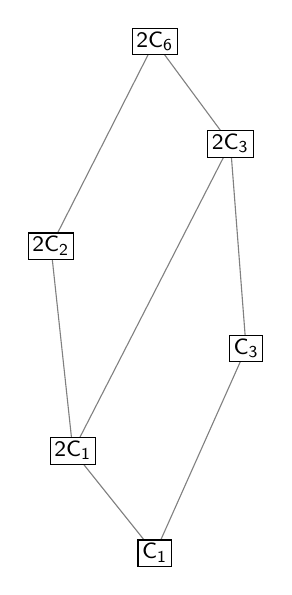
\begin{tikzpicture}[x=1cm, y=1.300cm,
  every node/.style={fill=white, font=\footnotesize, inner xsep=1.5pt, inner ysep=1.2pt, text height=5.6pt, text depth=1.6pt},
  normal/.style={draw, line width=0.4pt}, cover/.style={black!50, line width=0.4pt}]
\draw[cover] (0.00,0) -- (-1.04,1);
\draw[cover] (0.00,0) -- (1.16,2);
\draw[cover] (-1.04,1) -- (-1.32,3);
\draw[cover] (-1.04,1) -- (0.96,4);
\draw[cover] (1.16,2) -- (0.96,4);
\draw[cover] (-1.32,3) -- (0.00,5);
\draw[cover] (0.96,4) -- (0.00,5);
\node[normal] (n00) at (0.00,0) {$\grp{C_{1}}$};
\node[normal] (n01) at (-1.04,1) {$\grp{2C_{1}}$};
\node[normal] (n02) at (1.16,2) {$\grp{C_{3}}$};
\node[normal] (n03) at (-1.32,3) {$\grp{2C_{2}}$};
\node[normal] (n04) at (0.96,4) {$\grp{2C_{3}}$};
\node[normal] (n05) at (0.00,5) {$\grp{2C_{6}}$};
\end{tikzpicture}
\end{center}
{\small\setlength{\fillwidth}{\textwidth}\addtolength{\fillwidth}{-12\tabcolsep}\setlength{\colwidth}{0pt}\cellmax{$\grp{2C_{2}}$ $\samecls$ $\grp{2D_{1}}$}\cellmax{subgrp}\cellmax{$\grp{2C_{1}}$}\cellmax{$\grp{2C_{3}}$}\cellmax{$\grp{2C_{6}}$}\cellmax{$\grp{C_{1}}$}\cellmax{$\grp{C_{3}}$}\addtolength{\fillwidth}{-\colwidth}\setlength{\colwidth}{0pt}\cellmax{order}\cellmax{12}\cellmax{1}\cellmax{2}\cellmax{3}\cellmax{4}\cellmax{6}\addtolength{\fillwidth}{-\colwidth}\setlength{\colwidth}{0pt}\cellmax{conjugates}\cellmax{1}\addtolength{\fillwidth}{-\colwidth}\setlength{\colwidth}{0pt}\cellmax{normal}\cellmax{yes}\addtolength{\fillwidth}{-\colwidth}\setlength{\colwidth}{0pt}\cellmax{$\grp{N}_{\hairsp \grp{2C_{6}}}(\grp{H})$}\cellmax{$\grp{2C_{6}}$}\addtolength{\fillwidth}{-\colwidth}\setlength{\colwidth}{0pt}\cellmax{$\grp{C}_{\hairsp \grp{2C_{6}}}(\grp{H})$}\cellmax{$\grp{2C_{6}}$}\addtolength{\fillwidth}{-\colwidth}\setlength{\colwidth}{0pt}\cellmax{$\cls{\barred{E}}$, $\cls{C_{3}}$, $\cls{\barred{C}_{3}}$, $\cls{C_{3}^{2}}$, $\cls{\barred{C}_{3}^{2}}$}\cellmax{$\cls{\barred{E}}$, $\cls{C_{2}}$, $\cls{\barred{C}_{2}}$}\cellmax{$\cls{\barred{C}_{3}}$, $\cls{\barred{C}_{3}^{2}}$}\cellmax{classes}\cellmax{---}\cellmax{all}\cellmax{$\cls{\barred{E}}$}\fillcap\begin{longtable}{@{}lrrlll>{\RaggedRight\arraybackslash}p{\fillwidth}@{}}\toprule
subgrp & order & conjugates & normal & $\grp{N}_{\hairsp \grp{2C_{6}}}(\grp{H})$ & $\grp{C}_{\hairsp \grp{2C_{6}}}(\grp{H})$ & classes\\\midrule\endhead
\bottomrule\endfoot\endlastfoot
\href{C1.pdf}{$\grp{C_{1}}$} & 1 & 1 & yes & \href{2C6.pdf}{$\grp{2C_{6}}$} & \href{2C6.pdf}{$\grp{2C_{6}}$} & ---\\*
\href{2C1.pdf}{$\grp{2C_{1}}$} & 2 & 1 & yes & \href{2C6.pdf}{$\grp{2C_{6}}$} & \href{2C6.pdf}{$\grp{2C_{6}}$} & $\cls{\barred{E}}$\\
\href{C3.pdf}{$\grp{C_{3}}$} & 3 & 1 & yes & \href{2C6.pdf}{$\grp{2C_{6}}$} & \href{2C6.pdf}{$\grp{2C_{6}}$} & $\cls{\barred{C}_{3}}$, $\cls{\barred{C}_{3}^{2}}$\\
\href{2C2.pdf}{$\grp{2C_{2}}$} $\samecls$ \href{2D1.pdf}{$\grp{2D_{1}}$} & 4 & 1 & yes & \href{2C6.pdf}{$\grp{2C_{6}}$} & \href{2C6.pdf}{$\grp{2C_{6}}$} & $\cls{\barred{E}}$, $\cls{C_{2}}$, $\cls{\barred{C}_{2}}$\\
\href{2C3.pdf}{$\grp{2C_{3}}$} & 6 & 1 & yes & \href{2C6.pdf}{$\grp{2C_{6}}$} & \href{2C6.pdf}{$\grp{2C_{6}}$} & $\cls{\barred{E}}$, $\cls{C_{3}}$, $\cls{\barred{C}_{3}}$, $\cls{C_{3}^{2}}$, $\cls{\barred{C}_{3}^{2}}$\\*
\href{2C6.pdf}{$\grp{2C_{6}}$} & 12 & 1 & yes & \href{2C6.pdf}{$\grp{2C_{6}}$} & \href{2C6.pdf}{$\grp{2C_{6}}$} & all\\
\bottomrule\end{longtable}}
\needspace{103pt}
\section{Descent of symmetry}\label{s:subduction}
Conventions: \href{../../CONVENTIONS.pdf}{CONVENTIONS.pdf}, sections \href{../../../rotation/CONVENTIONS.pdf\#conv.12.2}{12.2}, \href{../../../rotation/CONVENTIONS.pdf\#conv.12.4}{12.4} and \href{../../CONVENTIONS.pdf\#conv.28}{28}.
A column is a class of subgroups $\grp{H}$, in the order of the table of section~\ref{s:subgroups}. The row subgrp names it by its symbol, as in that table. The symbol links to the document of $\grp{H}$. The entry of row $\Gamma$ is $\restr{\Gamma}{\grp{H}}$, the restriction of $\Gamma$ along a monomorphism from the record of $\grp{H}$ onto the subgroup, as a sum of the irreps of $\grp{H}$. The monomorphism identifies the subgroup with its record, and $\grp{H}$ names both. The rows of the vector irreps of a preimage are those of \href{../../../rotation/data/pdf/C6.pdf}{$\grp{C_{6}}$} (\texttt{vector\symbol{95}subduction}). The column of a section, which the record does not store, is that of its preimage with the spinor irreps renamed (\href{../../CONVENTIONS.pdf}{CONVENTIONS.pdf}, section \href{../../CONVENTIONS.pdf\#conv.27}{27}). \label{n:group.normalizer.o3}\label{n:group.centralizer.o3}\label{n:element.h}The record of $\grp{H}$ maps onto the subgroup in $\grpindex{\grp{N}}{\grp{C}}$ ways, $h \mapsto g h g^{-1}$ ($h \in \grp{H}$) for the $g \in \grp{Pin^{-}(3)}$ that carry $\grp{H}$ to it. Here $\grp{N}$ and $\grp{C}$ are the normalizer and centralizer of $\grp{H}$ in \href{Pinminus3.pdf}{$\grp{Pin^{-}(3)}$}. In the section Names and structure of the document of $\grp{H}$, the row centralizer gives $\grp{C}$ and the index $\grpindex{\grp{N}}{\grp{C}}$ (the index in the row normalizer is $\grpindex{\grp{N}}{\grp{H}}$). Two maps related by a conjugation in $\grp{2C_{6}}$ give the same restriction. Thus the maps fall into $\grpindex{\grp{N}}{\grp{C}}/\grpindex{\grp{N}_{\hairsp \grp{2C_{6}}}}{\grp{C}_{\hairsp \grp{2C_{6}}}}$ classes, where $\grp{N}_{\hairsp \grp{2C_{6}}}$ and $\grp{C}_{\hairsp \grp{2C_{6}}}$ are the normalizer and centralizer of the subgroup in $\grp{2C_{6}}$ (the table of section~\ref{s:subgroups}). \label{n:head.setting}A subgroup whose classes of maps give different tables has one column for each table: setting 1 for the stored monomorphism (\texttt{monomorphism}) and settings 2, 3, \dots{} for the \texttt{alternative\symbol{95}settings}. Each setting has the images of the generators of $\grp{H}$ (\texttt{setting}). \label{n:head.images}The row images gives, under each setting, each generator whose image differs between the settings, in their order, mapped to the class of $\grp{2C_{6}}$ that contains its image. Each generator is written by the symbol of its class (\href{../../CONVENTIONS.pdf}{CONVENTIONS.pdf}, section \href{../../../rotation/CONVENTIONS.pdf\#conv.5.1}{5.1}), and where two share a symbol, a superscript number in brackets gives the generator's index in the document of $\grp{H}$. \label{n:irrep.Delta}Each other setting is setting 1 with each irrep $\Lambda$ of $\grp{H}$ replaced by $\Lambda$ composed with one automorphism of $\grp{H}$ induced by a conjugation in \href{Pinminus3.pdf}{$\grp{Pin^{-}(3)}$} and by none in $\grp{2C_{6}}$ (\href{../../CONVENTIONS.pdf}{CONVENTIONS.pdf}, section \href{../../../rotation/CONVENTIONS.pdf\#conv.12.1}{12.1}).
{\small\begin{longtable}{@{}lcccccc@{}}\toprule
subgrp & \href{2C1.pdf}{$\grp{2C_{1}}$} & \href{C3.pdf}{$\grp{C_{3}}$} & \multicolumn{2}{c}{\href{2C2.pdf}{$\grp{2C_{2}}$}} & \multicolumn{2}{c}{\href{2C3.pdf}{$\grp{2C_{3}}$}}\\\cmidrule(lr){4-5}\cmidrule(lr){6-7}
setting &  &  & 1 & 2 & 1 & 2\\
images &  &  & {\scriptsize $\cls{C_{2}} \mapsto \cls{C_{2}}$} & {\scriptsize $\cls{C_{2}} \mapsto \cls{\barred{C}_{2}}$} & {\scriptsize $\cls{C_{3}} \mapsto \cls{C_{3}}$} & {\scriptsize $\cls{C_{3}} \mapsto \cls{C_{3}^{2}}$}\\\midrule\endhead
\bottomrule\endfoot\endlastfoot
$\irr{a}$ & $\irr{a}$ & $\irr{a}$ & $\irr{a}$ & $\irr{a}$ & $\irr{a}$ & $\irr{a}$\\*
$\irr{b}$ & $\irr{a}$ & $\irr{a}$ & $\irr{b}$ & $\irr{b}$ & $\irr{a}$ & $\irr{a}$\\*
$\conjpair{1}\irr{e}_{1}$ & $\irr{a}$ & $\conjpair{1}\irr{e}$ & $\irr{b}$ & $\irr{b}$ & $\conjpair{1}\irr{e}$ & $\conjpair{2}\irr{e}$\\*
$\conjpair{2}\irr{e}_{1}$ & $\irr{a}$ & $\conjpair{2}\irr{e}$ & $\irr{b}$ & $\irr{b}$ & $\conjpair{2}\irr{e}$ & $\conjpair{1}\irr{e}$\\*
$\conjpair{1}\irr{e}_{2}$ & $\irr{a}$ & $\conjpair{2}\irr{e}$ & $\irr{a}$ & $\irr{a}$ & $\conjpair{2}\irr{e}$ & $\conjpair{1}\irr{e}$\\*
$\conjpair{2}\irr{e}_{2}$ & $\irr{a}$ & $\conjpair{1}\irr{e}$ & $\irr{a}$ & $\irr{a}$ & $\conjpair{1}\irr{e}$ & $\conjpair{2}\irr{e}$\\*
$\conjpair{1}\irr{e}_{1/2}$ & $\irr{a}_{1/2}$ & $\conjpair{2}\irr{e}$ & $\conjpair{1}\irr{e}_{1/2}$ & $\conjpair{2}\irr{e}_{1/2}$ & $\conjpair{1}\irr{e}_{1/2}$ & $\conjpair{2}\irr{e}_{1/2}$\\*
$\conjpair{2}\irr{e}_{1/2}$ & $\irr{a}_{1/2}$ & $\conjpair{1}\irr{e}$ & $\conjpair{2}\irr{e}_{1/2}$ & $\conjpair{1}\irr{e}_{1/2}$ & $\conjpair{2}\irr{e}_{1/2}$ & $\conjpair{1}\irr{e}_{1/2}$\\*
$\conjpair{1}\irr{e}_{3/2}$ & $\irr{a}_{1/2}$ & $\irr{a}$ & $\conjpair{2}\irr{e}_{1/2}$ & $\conjpair{1}\irr{e}_{1/2}$ & $\irr{a}_{3/2}$ & $\irr{a}_{3/2}$\\*
$\conjpair{2}\irr{e}_{3/2}$ & $\irr{a}_{1/2}$ & $\irr{a}$ & $\conjpair{1}\irr{e}_{1/2}$ & $\conjpair{2}\irr{e}_{1/2}$ & $\irr{a}_{3/2}$ & $\irr{a}_{3/2}$\\*
$\conjpair{1}\irr{e}_{5/2}$ & $\irr{a}_{1/2}$ & $\conjpair{1}\irr{e}$ & $\conjpair{1}\irr{e}_{1/2}$ & $\conjpair{2}\irr{e}_{1/2}$ & $\conjpair{2}\irr{e}_{1/2}$ & $\conjpair{1}\irr{e}_{1/2}$\\*
$\conjpair{2}\irr{e}_{5/2}$ & $\irr{a}_{1/2}$ & $\conjpair{2}\irr{e}$ & $\conjpair{2}\irr{e}_{1/2}$ & $\conjpair{1}\irr{e}_{1/2}$ & $\conjpair{1}\irr{e}_{1/2}$ & $\conjpair{2}\irr{e}_{1/2}$\\
\bottomrule\end{longtable}}
Read down a column, a table gives induction (Frobenius reciprocity): $\Gamma$ occurs in $\Ind{\grp{H}}{\grp{2C_{6}}} \Lambda$ as often as $\Lambda$ occurs in the entry of row $\Gamma$. For every entry of a spinor irrep, the record holds the unitary matrix that carries $\restr{\Gamma}{\grp{H}}$ into the direct sum of the matrices of $\grp{H}$ (\texttt{subduction[].blocks}). For every class $\grp{H}$ it holds the left coset representatives (\texttt{transversal}). From both, $\Ind{\grp{H}}{\grp{2C_{6}}} \Lambda$ and its intertwiners follow as in \href{../../CONVENTIONS.pdf}{CONVENTIONS.pdf}, section \href{../../../rotation/CONVENTIONS.pdf\#conv.12.4}{12.4}.
\needspace{190pt}
\partbox{Angular momentum}
\section{Subduction from \texorpdfstring{$\grp{Pin^{-}(3)}$}{Pin\unichar{8315}(3)}}\label{s:subduction_parent}
Conventions: \href{../../CONVENTIONS.pdf}{CONVENTIONS.pdf}, sections \href{../../../rotation/CONVENTIONS.pdf\#conv.11}{11} and \href{../../CONVENTIONS.pdf\#conv.25.1}{25.1}.
\leavevmode\label{n:index.J}\label{n:index.parity}\label{n:irrep.o3}The irrep $\irrJp{J}{p}$ of \href{Pinminus3.pdf}{$\grp{Pin^{-}(3)}$} has angular momentum $J$ ($J = 0, \nicefrac{1}{2}, 1, \dots$) and parity $p$ ($\ptag{g}$ for $p = +1$, $\ptag{u}$ for $p = -1$). An element $(U, \varepsilon)$ acts on it as $\varepsilon^{[p = -1]}$ times $U$ acting on the kets of angular momentum $J$, and $\elt{\barred{E}}$ as $(-1)^{2J}$. \label{n:function.character.parent}\label{n:function.multiplicity}An element whose $\grp{SU(2)}$ part is $\lift{R}_{\vv}(\omega)$ (section~\ref{s:elements}) has the character
\begin{equation}\label{e:chi}\chi^{(J,p)}(g) = p^{\iverson{\det g = -1}}\sum_{m=-J}^{J} \expe^{\iunit m\omega},\end{equation}
and $b_\Gamma(J, p)$ is the multiplicity of $\Gamma$ in
\begin{equation}\label{e:parent}\restr{\irrJp{J}{p}}{\grp{2C_{6}}}.\end{equation}
At integer $J$ only the vector irreps occur, and $b_\Gamma(J, p)$ is the multiplicity in the subduction from $\grp{O(3)}$ to \href{../../../rotation/data/pdf/C6.pdf}{$\grp{C_{6}}$} (\texttt{integer\symbol{95}J}). \label{n:index.increment}At half-integer $J$ only the spinor irreps occur: each table gives $b_\Gamma(J, p)$ for $J \le \nicefrac{41}{2}$, and $b_\Gamma(J + 6, p) = b_\Gamma(J, p) + \Delta_\Gamma$ for every $J$, where $\Delta_\Gamma$ is the last row of the table of parity $p$. A table leaves out irreps of multiplicity 0 at every $J$.
\needspace{231pt}
\paragraph{Half-integer $J$, parity $\ptag{g}$ and $\ptag{u}$ ($p = \pm1$).}
Every element of $\grp{2C_{6}}$ covers a rotation, so the multiplicities do not depend on $p$ and one table gives both parities.
{\small\begin{longtable}{@{}rrrrrrr@{\hspace{18pt}}rrrrrrr@{}}\toprule
$J$ & $\conjpair{1}\irr{e}_{1/2}$ & $\conjpair{2}\irr{e}_{1/2}$ & $\conjpair{1}\irr{e}_{3/2}$ & $\conjpair{2}\irr{e}_{3/2}$ & $\conjpair{1}\irr{e}_{5/2}$ & $\conjpair{2}\irr{e}_{5/2}$ & $J$ & $\conjpair{1}\irr{e}_{1/2}$ & $\conjpair{2}\irr{e}_{1/2}$ & $\conjpair{1}\irr{e}_{3/2}$ & $\conjpair{2}\irr{e}_{3/2}$ & $\conjpair{1}\irr{e}_{5/2}$ & $\conjpair{2}\irr{e}_{5/2}$\\\midrule\endhead
\bottomrule\endfoot\endlastfoot
$\nicefrac{1}{2}$ & 1 & 1 & 0 & 0 & 0 & 0 & $\nicefrac{23}{2}$ & 4 & 4 & 4 & 4 & 4 & 4\\*
$\nicefrac{3}{2}$ & 1 & 1 & 1 & 1 & 0 & 0 & $\nicefrac{25}{2}$ & 5 & 5 & 4 & 4 & 4 & 4\\*
$\nicefrac{5}{2}$ & 1 & 1 & 1 & 1 & 1 & 1 & $\nicefrac{27}{2}$ & 5 & 5 & 5 & 5 & 4 & 4\\*
$\nicefrac{7}{2}$ & 1 & 1 & 1 & 1 & 2 & 2 & $\nicefrac{29}{2}$ & 5 & 5 & 5 & 5 & 5 & 5\\*
$\nicefrac{9}{2}$ & 1 & 1 & 2 & 2 & 2 & 2 & $\nicefrac{31}{2}$ & 5 & 5 & 5 & 5 & 6 & 6\\*
$\nicefrac{11}{2}$ & 2 & 2 & 2 & 2 & 2 & 2 & $\nicefrac{33}{2}$ & 5 & 5 & 6 & 6 & 6 & 6\\*
$\nicefrac{13}{2}$ & 3 & 3 & 2 & 2 & 2 & 2 & $\nicefrac{35}{2}$ & 6 & 6 & 6 & 6 & 6 & 6\\*
$\nicefrac{15}{2}$ & 3 & 3 & 3 & 3 & 2 & 2 & $\nicefrac{37}{2}$ & 7 & 7 & 6 & 6 & 6 & 6\\*
$\nicefrac{17}{2}$ & 3 & 3 & 3 & 3 & 3 & 3 & $\nicefrac{39}{2}$ & 7 & 7 & 7 & 7 & 6 & 6\\*
$\nicefrac{19}{2}$ & 3 & 3 & 3 & 3 & 4 & 4 & $\nicefrac{41}{2}$ & 7 & 7 & 7 & 7 & 7 & 7\\*\noalign{\vskip 1.5pt}\multispan{7} & \multispan{7}\leaders\hrule height\cmidrulewidth\hfill\kern0pt\\*\noalign{\vskip 1.5pt}
$\nicefrac{21}{2}$ & 3 & 3 & 4 & 4 & 4 & 4 & $\Delta_\Gamma$ & 2 & 2 & 2 & 2 & 2 & 2\\
\bottomrule\end{longtable}}
\needspace{110pt}
\section{Multiplicities and allowed \texorpdfstring{$m$}{m}}\label{s:multiplicities}
Conventions: \href{../../CONVENTIONS.pdf}{CONVENTIONS.pdf}, sections \href{../../../rotation/CONVENTIONS.pdf\#conv.14}{14} and \href{../../CONVENTIONS.pdf\#conv.26}{26}.
\leavevmode\label{n:function.generating}\label{n:index.generating.variable}\label{n:function.generating.numerator}The multiplicity $b_\Gamma(J) = b_\Gamma(J, +1)$ is the number of blocks of $\Gamma$ at $J$, with the generating function
\begin{equation}\label{e:gf}H_\Gamma(t) = \sum_{J\ge1/2} b_\Gamma(J)\,t^{2J} = P_\Gamma(t)/((1-t^{2})(1-t^{12})),\end{equation}
summed over the half-integer $J$. \label{n:delimiter.floor}\label{n:local.floor.x}The floor $\lfloor x\rfloor$ is the greatest integer $\le x$. The listed residues are the $2m \bmod 12$ of the nonzero components of the vectors of $\Gamma$.
{\small{\renewcommand{\arraystretch}{1.3}\begin{longtable}{@{}llll@{}}\toprule
$\Gamma$ & $P_\Gamma(t)$ & $b_\Gamma(J)$ & $2m \bmod 12$\\\midrule\endhead
\bottomrule\endfoot\endlastfoot
$\conjpair{1}\irr{e}_{1/2}$ & $t + t^{11}$ & $\bigl\lfloor\tfrac{2J}{12}\bigr\rfloor + \bigl\lfloor\tfrac{2J+1}{12}\bigr\rfloor + 1$ & 1\\*
$\conjpair{2}\irr{e}_{1/2}$ & $t + t^{11}$ & $\bigl\lfloor\tfrac{2J}{12}\bigr\rfloor + \bigl\lfloor\tfrac{2J+1}{12}\bigr\rfloor + 1$ & 11\\*
$\conjpair{1}\irr{e}_{3/2}$ & $t^{3} + t^{9}$ & $\bigl\lfloor\tfrac{2J+3}{6}\bigr\rfloor$ & 3\\*
$\conjpair{2}\irr{e}_{3/2}$ & $t^{3} + t^{9}$ & $\bigl\lfloor\tfrac{2J+3}{6}\bigr\rfloor$ & 9\\*
$\conjpair{1}\irr{e}_{5/2}$ & $t^{5} + t^{7}$ & $\bigl\lfloor\tfrac{2J+5}{12}\bigr\rfloor + \bigl\lfloor\tfrac{2J+7}{12}\bigr\rfloor$ & 5\\*
$\conjpair{2}\irr{e}_{5/2}$ & $t^{5} + t^{7}$ & $\bigl\lfloor\tfrac{2J+5}{12}\bigr\rfloor + \bigl\lfloor\tfrac{2J+7}{12}\bigr\rfloor$ & 7\\
\bottomrule\end{longtable}}}
\needspace{122pt}
\section{Symmetry-adapted bases}\label{s:bases}
Conventions: \href{../../CONVENTIONS.pdf}{CONVENTIONS.pdf}, sections \href{../../../rotation/CONVENTIONS.pdf\#conv.14}{14} and \href{../../CONVENTIONS.pdf\#conv.26}{26}.
\leavevmode\label{n:index.m}\label{n:vector.ket}The bases at integer $J$ are those of \href{../../../rotation/data/pdf/C6.pdf}{$\grp{C_{6}}$} (\texttt{integer\symbol{95}J}), and at half-integer $J$ the kets $\jm{J}{m}$, $m = J, J-1, \dots, -J$, carry $\irrJp{J}{+1}$. \label{n:matrix.wigner}The Wigner matrix $\wignerD{J}$ of $\grp{SU(2)}$ satisfies $\wignerD{1/2}(U) = U$ on $\jm{1/2}{1/2}$, $\jm{1/2}{-1/2}$. The element $g$ of $\grp{2C_{6}}$ whose $\grp{SU(2)}$ part is $U$ acts as
\begin{equation}\label{e:action}g\,\jm{J}{m} = \sum_{m'} \jm{J}{m'}\; \conj{\wignerD{J}_{m m'}(U)},\end{equation}
so $\lift{R}_{z}(\omega)$ multiplies $\jm{J}{m}$ by $\expe^{\iunit m\omega}$, $0 \le \omega < 4\pi$, and $\elt{\barred{E}}$ by $-1$. \label{n:index.ketcoefficient}\label{n:vector.basis.symmetry}\label{n:index.ketweight}\label{n:index.total}A vector is listed by its coefficients $e_m$:
\begin{equation}\label{e:ket}v = \frac{1}{\sqrt{\mathrm{tot}}}\sum_m e_m\sqrt{F_m}\;\jm{J}{m},\qquad F_m = (J+m)!\,(J-m)!,\qquad \mathrm{tot} = \sum_m |e_m|^2F_m,\end{equation}
so every $e_m$ here is $\pm 1$.
\leavevmode\label{n:group.A}The subgroup $\grp{A}$ of the elements over $\grp{C_{\infty h}}$ acts diagonally on the kets, and $\grp{2C_{6}} = \grp{A}$: every ket is a block. Blocks are ordered by $J$, then $|m|$, $+m$ before $-m$.
The bases have 132 blocks and 132 vectors at $J = \nicefrac{1}{2}, \nicefrac{3}{2}, \dots, \nicefrac{21}{2}$. \label{n:index.copy}\label{n:head.vector}A row gives a vector of a block at $J$: the block's irrep and copy index $\mult$, the partner index $\intx$ and the vector.
{\small\setlength{\tabcolsep}{3pt}\begin{longtable}{@{}rlrr@{\hspace{4pt}}l@{\hspace{18pt}}rlrr@{\hspace{4pt}}l@{}}\toprule
$J$ & irrep & $\mult$ & $\intx$ & vector & $J$ & irrep & $\mult$ & $\intx$ & vector\\\midrule\endhead
\bottomrule\endfoot\endlastfoot
$\nicefrac{1}{2}$ & $\conjpair{1}\irr{e}_{1/2}$ & 1 & 1 & $\jm{\nicefrac{1}{2}}{\nicefrac{1}{2}}$ & $\nicefrac{5}{2}$ & $\conjpair{2}\irr{e}_{5/2}$ & 1 & 1 & $\jm{\nicefrac{5}{2}}{-\nicefrac{5}{2}}$\\*\noalign{\vskip 1.5pt}\multispan{5} & \multispan{5}\leaders\hrule height\cmidrulewidth\hfill\kern0pt\\*\noalign{\vskip 1.5pt}
$\nicefrac{1}{2}$ & $\conjpair{2}\irr{e}_{1/2}$ & 1 & 1 & $\jm{\nicefrac{1}{2}}{-\nicefrac{1}{2}}$ & $\nicefrac{7}{2}$ & $\conjpair{1}\irr{e}_{1/2}$ & 1 & 1 & $\jm{\nicefrac{7}{2}}{\nicefrac{1}{2}}$\\*\noalign{\vskip 1.5pt}\multispan{5}\leaders\hrule height\cmidrulewidth\hfill\kern0pt\hskip18pt & \multispan{5}\\*\noalign{\vskip 1.5pt}
$\nicefrac{3}{2}$ & $\conjpair{1}\irr{e}_{1/2}$ & 1 & 1 & $\jm{\nicefrac{3}{2}}{\nicefrac{1}{2}}$ & $\nicefrac{7}{2}$ & $\conjpair{2}\irr{e}_{1/2}$ & 1 & 1 & $\jm{\nicefrac{7}{2}}{-\nicefrac{1}{2}}$\\*
$\nicefrac{3}{2}$ & $\conjpair{2}\irr{e}_{1/2}$ & 1 & 1 & $\jm{\nicefrac{3}{2}}{-\nicefrac{1}{2}}$ & $\nicefrac{7}{2}$ & $\conjpair{1}\irr{e}_{3/2}$ & 1 & 1 & $\jm{\nicefrac{7}{2}}{\nicefrac{3}{2}}$\\*
$\nicefrac{3}{2}$ & $\conjpair{1}\irr{e}_{3/2}$ & 1 & 1 & $\jm{\nicefrac{3}{2}}{\nicefrac{3}{2}}$ & $\nicefrac{7}{2}$ & $\conjpair{2}\irr{e}_{3/2}$ & 1 & 1 & $\jm{\nicefrac{7}{2}}{-\nicefrac{3}{2}}$\\*
$\nicefrac{3}{2}$ & $\conjpair{2}\irr{e}_{3/2}$ & 1 & 1 & $\jm{\nicefrac{3}{2}}{-\nicefrac{3}{2}}$ & $\nicefrac{7}{2}$ & $\conjpair{1}\irr{e}_{5/2}$ & 1 & 1 & $\jm{\nicefrac{7}{2}}{\nicefrac{5}{2}}$\\*\noalign{\vskip 1.5pt}\multispan{5}\leaders\hrule height\cmidrulewidth\hfill\kern0pt\hskip18pt & \multispan{5}\\*\noalign{\vskip 1.5pt}
$\nicefrac{5}{2}$ & $\conjpair{1}\irr{e}_{1/2}$ & 1 & 1 & $\jm{\nicefrac{5}{2}}{\nicefrac{1}{2}}$ & $\nicefrac{7}{2}$ & $\conjpair{2}\irr{e}_{5/2}$ & 1 & 1 & $\jm{\nicefrac{7}{2}}{-\nicefrac{5}{2}}$\\*
$\nicefrac{5}{2}$ & $\conjpair{2}\irr{e}_{1/2}$ & 1 & 1 & $\jm{\nicefrac{5}{2}}{-\nicefrac{1}{2}}$ & $\nicefrac{7}{2}$ & $\conjpair{2}\irr{e}_{5/2}$ & 2 & 1 & $\jm{\nicefrac{7}{2}}{\nicefrac{7}{2}}$\\*
$\nicefrac{5}{2}$ & $\conjpair{1}\irr{e}_{3/2}$ & 1 & 1 & $\jm{\nicefrac{5}{2}}{\nicefrac{3}{2}}$ & $\nicefrac{7}{2}$ & $\conjpair{1}\irr{e}_{5/2}$ & 2 & 1 & $\jm{\nicefrac{7}{2}}{-\nicefrac{7}{2}}$\\*\noalign{\vskip 1.5pt}\multispan{5} & \multispan{5}\leaders\hrule height\cmidrulewidth\hfill\kern0pt\\*\noalign{\vskip 1.5pt}
$\nicefrac{5}{2}$ & $\conjpair{2}\irr{e}_{3/2}$ & 1 & 1 & $\jm{\nicefrac{5}{2}}{-\nicefrac{3}{2}}$ & $\nicefrac{9}{2}$ & $\conjpair{1}\irr{e}_{1/2}$ & 1 & 1 & $\jm{\nicefrac{9}{2}}{\nicefrac{1}{2}}$\\*
$\nicefrac{5}{2}$ & $\conjpair{1}\irr{e}_{5/2}$ & 1 & 1 & $\jm{\nicefrac{5}{2}}{\nicefrac{5}{2}}$ & $\nicefrac{9}{2}$ & $\conjpair{2}\irr{e}_{1/2}$ & 1 & 1 & $\jm{\nicefrac{9}{2}}{-\nicefrac{1}{2}}$\\
\grouprule{0pt}{\heavyrulewidth}
$\nicefrac{9}{2}$ & $\conjpair{1}\irr{e}_{3/2}$ & 1 & 1 & $\jm{\nicefrac{9}{2}}{\nicefrac{3}{2}}$ & $\nicefrac{11}{2}$ & $\conjpair{2}\irr{e}_{3/2}$ & 1 & 1 & $\jm{\nicefrac{11}{2}}{-\nicefrac{3}{2}}$\\*
$\nicefrac{9}{2}$ & $\conjpair{2}\irr{e}_{3/2}$ & 1 & 1 & $\jm{\nicefrac{9}{2}}{-\nicefrac{3}{2}}$ & $\nicefrac{11}{2}$ & $\conjpair{1}\irr{e}_{5/2}$ & 1 & 1 & $\jm{\nicefrac{11}{2}}{\nicefrac{5}{2}}$\\*
$\nicefrac{9}{2}$ & $\conjpair{1}\irr{e}_{5/2}$ & 1 & 1 & $\jm{\nicefrac{9}{2}}{\nicefrac{5}{2}}$ & $\nicefrac{11}{2}$ & $\conjpair{2}\irr{e}_{5/2}$ & 1 & 1 & $\jm{\nicefrac{11}{2}}{-\nicefrac{5}{2}}$\\*
$\nicefrac{9}{2}$ & $\conjpair{2}\irr{e}_{5/2}$ & 1 & 1 & $\jm{\nicefrac{9}{2}}{-\nicefrac{5}{2}}$ & $\nicefrac{11}{2}$ & $\conjpair{2}\irr{e}_{5/2}$ & 2 & 1 & $\jm{\nicefrac{11}{2}}{\nicefrac{7}{2}}$\\*
$\nicefrac{9}{2}$ & $\conjpair{2}\irr{e}_{5/2}$ & 2 & 1 & $\jm{\nicefrac{9}{2}}{\nicefrac{7}{2}}$ & $\nicefrac{11}{2}$ & $\conjpair{1}\irr{e}_{5/2}$ & 2 & 1 & $\jm{\nicefrac{11}{2}}{-\nicefrac{7}{2}}$\\*
$\nicefrac{9}{2}$ & $\conjpair{1}\irr{e}_{5/2}$ & 2 & 1 & $\jm{\nicefrac{9}{2}}{-\nicefrac{7}{2}}$ & $\nicefrac{11}{2}$ & $\conjpair{2}\irr{e}_{3/2}$ & 2 & 1 & $\jm{\nicefrac{11}{2}}{\nicefrac{9}{2}}$\\*
$\nicefrac{9}{2}$ & $\conjpair{2}\irr{e}_{3/2}$ & 2 & 1 & $\jm{\nicefrac{9}{2}}{\nicefrac{9}{2}}$ & $\nicefrac{11}{2}$ & $\conjpair{1}\irr{e}_{3/2}$ & 2 & 1 & $\jm{\nicefrac{11}{2}}{-\nicefrac{9}{2}}$\\*
$\nicefrac{9}{2}$ & $\conjpair{1}\irr{e}_{3/2}$ & 2 & 1 & $\jm{\nicefrac{9}{2}}{-\nicefrac{9}{2}}$ & $\nicefrac{11}{2}$ & $\conjpair{2}\irr{e}_{1/2}$ & 2 & 1 & $\jm{\nicefrac{11}{2}}{\nicefrac{11}{2}}$\\*\noalign{\vskip 1.5pt}\multispan{5}\leaders\hrule height\cmidrulewidth\hfill\kern0pt\hskip18pt & \multispan{5}\\*\noalign{\vskip 1.5pt}
$\nicefrac{11}{2}$ & $\conjpair{1}\irr{e}_{1/2}$ & 1 & 1 & $\jm{\nicefrac{11}{2}}{\nicefrac{1}{2}}$ & $\nicefrac{11}{2}$ & $\conjpair{1}\irr{e}_{1/2}$ & 2 & 1 & $\jm{\nicefrac{11}{2}}{-\nicefrac{11}{2}}$\\*\noalign{\vskip 1.5pt}\multispan{5} & \multispan{5}\leaders\hrule height\cmidrulewidth\hfill\kern0pt\\*\noalign{\vskip 1.5pt}
$\nicefrac{11}{2}$ & $\conjpair{2}\irr{e}_{1/2}$ & 1 & 1 & $\jm{\nicefrac{11}{2}}{-\nicefrac{1}{2}}$ & $\nicefrac{13}{2}$ & $\conjpair{1}\irr{e}_{1/2}$ & 1 & 1 & $\jm{\nicefrac{13}{2}}{\nicefrac{1}{2}}$\\*
$\nicefrac{11}{2}$ & $\conjpair{1}\irr{e}_{3/2}$ & 1 & 1 & $\jm{\nicefrac{11}{2}}{\nicefrac{3}{2}}$ & $\nicefrac{13}{2}$ & $\conjpair{2}\irr{e}_{1/2}$ & 1 & 1 & $\jm{\nicefrac{13}{2}}{-\nicefrac{1}{2}}$\\
\grouprule{0pt}{\heavyrulewidth}
$\nicefrac{13}{2}$ & $\conjpair{1}\irr{e}_{3/2}$ & 1 & 1 & $\jm{\nicefrac{13}{2}}{\nicefrac{3}{2}}$ & $\nicefrac{13}{2}$ & $\conjpair{2}\irr{e}_{1/2}$ & 3 & 1 & $\jm{\nicefrac{13}{2}}{-\nicefrac{13}{2}}$\\*\noalign{\vskip 1.5pt}\multispan{5} & \multispan{5}\leaders\hrule height\cmidrulewidth\hfill\kern0pt\\*\noalign{\vskip 1.5pt}
$\nicefrac{13}{2}$ & $\conjpair{2}\irr{e}_{3/2}$ & 1 & 1 & $\jm{\nicefrac{13}{2}}{-\nicefrac{3}{2}}$ & $\nicefrac{15}{2}$ & $\conjpair{1}\irr{e}_{1/2}$ & 1 & 1 & $\jm{\nicefrac{15}{2}}{\nicefrac{1}{2}}$\\*
$\nicefrac{13}{2}$ & $\conjpair{1}\irr{e}_{5/2}$ & 1 & 1 & $\jm{\nicefrac{13}{2}}{\nicefrac{5}{2}}$ & $\nicefrac{15}{2}$ & $\conjpair{2}\irr{e}_{1/2}$ & 1 & 1 & $\jm{\nicefrac{15}{2}}{-\nicefrac{1}{2}}$\\*
$\nicefrac{13}{2}$ & $\conjpair{2}\irr{e}_{5/2}$ & 1 & 1 & $\jm{\nicefrac{13}{2}}{-\nicefrac{5}{2}}$ & $\nicefrac{15}{2}$ & $\conjpair{1}\irr{e}_{3/2}$ & 1 & 1 & $\jm{\nicefrac{15}{2}}{\nicefrac{3}{2}}$\\*
$\nicefrac{13}{2}$ & $\conjpair{2}\irr{e}_{5/2}$ & 2 & 1 & $\jm{\nicefrac{13}{2}}{\nicefrac{7}{2}}$ & $\nicefrac{15}{2}$ & $\conjpair{2}\irr{e}_{3/2}$ & 1 & 1 & $\jm{\nicefrac{15}{2}}{-\nicefrac{3}{2}}$\\*
$\nicefrac{13}{2}$ & $\conjpair{1}\irr{e}_{5/2}$ & 2 & 1 & $\jm{\nicefrac{13}{2}}{-\nicefrac{7}{2}}$ & $\nicefrac{15}{2}$ & $\conjpair{1}\irr{e}_{5/2}$ & 1 & 1 & $\jm{\nicefrac{15}{2}}{\nicefrac{5}{2}}$\\*
$\nicefrac{13}{2}$ & $\conjpair{2}\irr{e}_{3/2}$ & 2 & 1 & $\jm{\nicefrac{13}{2}}{\nicefrac{9}{2}}$ & $\nicefrac{15}{2}$ & $\conjpair{2}\irr{e}_{5/2}$ & 1 & 1 & $\jm{\nicefrac{15}{2}}{-\nicefrac{5}{2}}$\\*
$\nicefrac{13}{2}$ & $\conjpair{1}\irr{e}_{3/2}$ & 2 & 1 & $\jm{\nicefrac{13}{2}}{-\nicefrac{9}{2}}$ & $\nicefrac{15}{2}$ & $\conjpair{2}\irr{e}_{5/2}$ & 2 & 1 & $\jm{\nicefrac{15}{2}}{\nicefrac{7}{2}}$\\*
$\nicefrac{13}{2}$ & $\conjpair{2}\irr{e}_{1/2}$ & 2 & 1 & $\jm{\nicefrac{13}{2}}{\nicefrac{11}{2}}$ & $\nicefrac{15}{2}$ & $\conjpair{1}\irr{e}_{5/2}$ & 2 & 1 & $\jm{\nicefrac{15}{2}}{-\nicefrac{7}{2}}$\\*
$\nicefrac{13}{2}$ & $\conjpair{1}\irr{e}_{1/2}$ & 2 & 1 & $\jm{\nicefrac{13}{2}}{-\nicefrac{11}{2}}$ & $\nicefrac{15}{2}$ & $\conjpair{2}\irr{e}_{3/2}$ & 2 & 1 & $\jm{\nicefrac{15}{2}}{\nicefrac{9}{2}}$\\*
$\nicefrac{13}{2}$ & $\conjpair{1}\irr{e}_{1/2}$ & 3 & 1 & $\jm{\nicefrac{13}{2}}{\nicefrac{13}{2}}$ & $\nicefrac{15}{2}$ & $\conjpair{1}\irr{e}_{3/2}$ & 2 & 1 & $\jm{\nicefrac{15}{2}}{-\nicefrac{9}{2}}$\\
\grouprule{0pt}{\heavyrulewidth}
$\nicefrac{15}{2}$ & $\conjpair{2}\irr{e}_{1/2}$ & 2 & 1 & $\jm{\nicefrac{15}{2}}{\nicefrac{11}{2}}$ & $\nicefrac{17}{2}$ & $\conjpair{2}\irr{e}_{5/2}$ & 1 & 1 & $\jm{\nicefrac{17}{2}}{-\nicefrac{5}{2}}$\\*
$\nicefrac{15}{2}$ & $\conjpair{1}\irr{e}_{1/2}$ & 2 & 1 & $\jm{\nicefrac{15}{2}}{-\nicefrac{11}{2}}$ & $\nicefrac{17}{2}$ & $\conjpair{2}\irr{e}_{5/2}$ & 2 & 1 & $\jm{\nicefrac{17}{2}}{\nicefrac{7}{2}}$\\*
$\nicefrac{15}{2}$ & $\conjpair{1}\irr{e}_{1/2}$ & 3 & 1 & $\jm{\nicefrac{15}{2}}{\nicefrac{13}{2}}$ & $\nicefrac{17}{2}$ & $\conjpair{1}\irr{e}_{5/2}$ & 2 & 1 & $\jm{\nicefrac{17}{2}}{-\nicefrac{7}{2}}$\\*
$\nicefrac{15}{2}$ & $\conjpair{2}\irr{e}_{1/2}$ & 3 & 1 & $\jm{\nicefrac{15}{2}}{-\nicefrac{13}{2}}$ & $\nicefrac{17}{2}$ & $\conjpair{2}\irr{e}_{3/2}$ & 2 & 1 & $\jm{\nicefrac{17}{2}}{\nicefrac{9}{2}}$\\*
$\nicefrac{15}{2}$ & $\conjpair{1}\irr{e}_{3/2}$ & 3 & 1 & $\jm{\nicefrac{15}{2}}{\nicefrac{15}{2}}$ & $\nicefrac{17}{2}$ & $\conjpair{1}\irr{e}_{3/2}$ & 2 & 1 & $\jm{\nicefrac{17}{2}}{-\nicefrac{9}{2}}$\\*
$\nicefrac{15}{2}$ & $\conjpair{2}\irr{e}_{3/2}$ & 3 & 1 & $\jm{\nicefrac{15}{2}}{-\nicefrac{15}{2}}$ & $\nicefrac{17}{2}$ & $\conjpair{2}\irr{e}_{1/2}$ & 2 & 1 & $\jm{\nicefrac{17}{2}}{\nicefrac{11}{2}}$\\*\noalign{\vskip 1.5pt}\multispan{5}\leaders\hrule height\cmidrulewidth\hfill\kern0pt\hskip18pt & \multispan{5}\\*\noalign{\vskip 1.5pt}
$\nicefrac{17}{2}$ & $\conjpair{1}\irr{e}_{1/2}$ & 1 & 1 & $\jm{\nicefrac{17}{2}}{\nicefrac{1}{2}}$ & $\nicefrac{17}{2}$ & $\conjpair{1}\irr{e}_{1/2}$ & 2 & 1 & $\jm{\nicefrac{17}{2}}{-\nicefrac{11}{2}}$\\*
$\nicefrac{17}{2}$ & $\conjpair{2}\irr{e}_{1/2}$ & 1 & 1 & $\jm{\nicefrac{17}{2}}{-\nicefrac{1}{2}}$ & $\nicefrac{17}{2}$ & $\conjpair{1}\irr{e}_{1/2}$ & 3 & 1 & $\jm{\nicefrac{17}{2}}{\nicefrac{13}{2}}$\\*
$\nicefrac{17}{2}$ & $\conjpair{1}\irr{e}_{3/2}$ & 1 & 1 & $\jm{\nicefrac{17}{2}}{\nicefrac{3}{2}}$ & $\nicefrac{17}{2}$ & $\conjpair{2}\irr{e}_{1/2}$ & 3 & 1 & $\jm{\nicefrac{17}{2}}{-\nicefrac{13}{2}}$\\*
$\nicefrac{17}{2}$ & $\conjpair{2}\irr{e}_{3/2}$ & 1 & 1 & $\jm{\nicefrac{17}{2}}{-\nicefrac{3}{2}}$ & $\nicefrac{17}{2}$ & $\conjpair{1}\irr{e}_{3/2}$ & 3 & 1 & $\jm{\nicefrac{17}{2}}{\nicefrac{15}{2}}$\\*
$\nicefrac{17}{2}$ & $\conjpair{1}\irr{e}_{5/2}$ & 1 & 1 & $\jm{\nicefrac{17}{2}}{\nicefrac{5}{2}}$ & $\nicefrac{17}{2}$ & $\conjpair{2}\irr{e}_{3/2}$ & 3 & 1 & $\jm{\nicefrac{17}{2}}{-\nicefrac{15}{2}}$\\
\grouprule{0pt}{\heavyrulewidth}
$\nicefrac{17}{2}$ & $\conjpair{1}\irr{e}_{5/2}$ & 3 & 1 & $\jm{\nicefrac{17}{2}}{\nicefrac{17}{2}}$ & $\nicefrac{19}{2}$ & $\conjpair{1}\irr{e}_{3/2}$ & 2 & 1 & $\jm{\nicefrac{19}{2}}{-\nicefrac{9}{2}}$\\*
$\nicefrac{17}{2}$ & $\conjpair{2}\irr{e}_{5/2}$ & 3 & 1 & $\jm{\nicefrac{17}{2}}{-\nicefrac{17}{2}}$ & $\nicefrac{19}{2}$ & $\conjpair{2}\irr{e}_{1/2}$ & 2 & 1 & $\jm{\nicefrac{19}{2}}{\nicefrac{11}{2}}$\\*\noalign{\vskip 1.5pt}\multispan{5}\leaders\hrule height\cmidrulewidth\hfill\kern0pt\hskip18pt & \multispan{5}\\*\noalign{\vskip 1.5pt}
$\nicefrac{19}{2}$ & $\conjpair{1}\irr{e}_{1/2}$ & 1 & 1 & $\jm{\nicefrac{19}{2}}{\nicefrac{1}{2}}$ & $\nicefrac{19}{2}$ & $\conjpair{1}\irr{e}_{1/2}$ & 2 & 1 & $\jm{\nicefrac{19}{2}}{-\nicefrac{11}{2}}$\\*
$\nicefrac{19}{2}$ & $\conjpair{2}\irr{e}_{1/2}$ & 1 & 1 & $\jm{\nicefrac{19}{2}}{-\nicefrac{1}{2}}$ & $\nicefrac{19}{2}$ & $\conjpair{1}\irr{e}_{1/2}$ & 3 & 1 & $\jm{\nicefrac{19}{2}}{\nicefrac{13}{2}}$\\*
$\nicefrac{19}{2}$ & $\conjpair{1}\irr{e}_{3/2}$ & 1 & 1 & $\jm{\nicefrac{19}{2}}{\nicefrac{3}{2}}$ & $\nicefrac{19}{2}$ & $\conjpair{2}\irr{e}_{1/2}$ & 3 & 1 & $\jm{\nicefrac{19}{2}}{-\nicefrac{13}{2}}$\\*
$\nicefrac{19}{2}$ & $\conjpair{2}\irr{e}_{3/2}$ & 1 & 1 & $\jm{\nicefrac{19}{2}}{-\nicefrac{3}{2}}$ & $\nicefrac{19}{2}$ & $\conjpair{1}\irr{e}_{3/2}$ & 3 & 1 & $\jm{\nicefrac{19}{2}}{\nicefrac{15}{2}}$\\*
$\nicefrac{19}{2}$ & $\conjpair{1}\irr{e}_{5/2}$ & 1 & 1 & $\jm{\nicefrac{19}{2}}{\nicefrac{5}{2}}$ & $\nicefrac{19}{2}$ & $\conjpair{2}\irr{e}_{3/2}$ & 3 & 1 & $\jm{\nicefrac{19}{2}}{-\nicefrac{15}{2}}$\\*
$\nicefrac{19}{2}$ & $\conjpair{2}\irr{e}_{5/2}$ & 1 & 1 & $\jm{\nicefrac{19}{2}}{-\nicefrac{5}{2}}$ & $\nicefrac{19}{2}$ & $\conjpair{1}\irr{e}_{5/2}$ & 3 & 1 & $\jm{\nicefrac{19}{2}}{\nicefrac{17}{2}}$\\*
$\nicefrac{19}{2}$ & $\conjpair{2}\irr{e}_{5/2}$ & 2 & 1 & $\jm{\nicefrac{19}{2}}{\nicefrac{7}{2}}$ & $\nicefrac{19}{2}$ & $\conjpair{2}\irr{e}_{5/2}$ & 3 & 1 & $\jm{\nicefrac{19}{2}}{-\nicefrac{17}{2}}$\\*
$\nicefrac{19}{2}$ & $\conjpair{1}\irr{e}_{5/2}$ & 2 & 1 & $\jm{\nicefrac{19}{2}}{-\nicefrac{7}{2}}$ & $\nicefrac{19}{2}$ & $\conjpair{2}\irr{e}_{5/2}$ & 4 & 1 & $\jm{\nicefrac{19}{2}}{\nicefrac{19}{2}}$\\*
$\nicefrac{19}{2}$ & $\conjpair{2}\irr{e}_{3/2}$ & 2 & 1 & $\jm{\nicefrac{19}{2}}{\nicefrac{9}{2}}$ & $\nicefrac{19}{2}$ & $\conjpair{1}\irr{e}_{5/2}$ & 4 & 1 & $\jm{\nicefrac{19}{2}}{-\nicefrac{19}{2}}$\\
\grouprule{0pt}{\heavyrulewidth}
$\nicefrac{21}{2}$ & $\conjpair{1}\irr{e}_{1/2}$ & 1 & 1 & $\jm{\nicefrac{21}{2}}{\nicefrac{1}{2}}$ & $\nicefrac{21}{2}$ & $\conjpair{1}\irr{e}_{1/2}$ & 2 & 1 & $\jm{\nicefrac{21}{2}}{-\nicefrac{11}{2}}$\\*
$\nicefrac{21}{2}$ & $\conjpair{2}\irr{e}_{1/2}$ & 1 & 1 & $\jm{\nicefrac{21}{2}}{-\nicefrac{1}{2}}$ & $\nicefrac{21}{2}$ & $\conjpair{1}\irr{e}_{1/2}$ & 3 & 1 & $\jm{\nicefrac{21}{2}}{\nicefrac{13}{2}}$\\*
$\nicefrac{21}{2}$ & $\conjpair{1}\irr{e}_{3/2}$ & 1 & 1 & $\jm{\nicefrac{21}{2}}{\nicefrac{3}{2}}$ & $\nicefrac{21}{2}$ & $\conjpair{2}\irr{e}_{1/2}$ & 3 & 1 & $\jm{\nicefrac{21}{2}}{-\nicefrac{13}{2}}$\\*
$\nicefrac{21}{2}$ & $\conjpair{2}\irr{e}_{3/2}$ & 1 & 1 & $\jm{\nicefrac{21}{2}}{-\nicefrac{3}{2}}$ & $\nicefrac{21}{2}$ & $\conjpair{1}\irr{e}_{3/2}$ & 3 & 1 & $\jm{\nicefrac{21}{2}}{\nicefrac{15}{2}}$\\*
$\nicefrac{21}{2}$ & $\conjpair{1}\irr{e}_{5/2}$ & 1 & 1 & $\jm{\nicefrac{21}{2}}{\nicefrac{5}{2}}$ & $\nicefrac{21}{2}$ & $\conjpair{2}\irr{e}_{3/2}$ & 3 & 1 & $\jm{\nicefrac{21}{2}}{-\nicefrac{15}{2}}$\\*
$\nicefrac{21}{2}$ & $\conjpair{2}\irr{e}_{5/2}$ & 1 & 1 & $\jm{\nicefrac{21}{2}}{-\nicefrac{5}{2}}$ & $\nicefrac{21}{2}$ & $\conjpair{1}\irr{e}_{5/2}$ & 3 & 1 & $\jm{\nicefrac{21}{2}}{\nicefrac{17}{2}}$\\*
$\nicefrac{21}{2}$ & $\conjpair{2}\irr{e}_{5/2}$ & 2 & 1 & $\jm{\nicefrac{21}{2}}{\nicefrac{7}{2}}$ & $\nicefrac{21}{2}$ & $\conjpair{2}\irr{e}_{5/2}$ & 3 & 1 & $\jm{\nicefrac{21}{2}}{-\nicefrac{17}{2}}$\\*
$\nicefrac{21}{2}$ & $\conjpair{1}\irr{e}_{5/2}$ & 2 & 1 & $\jm{\nicefrac{21}{2}}{-\nicefrac{7}{2}}$ & $\nicefrac{21}{2}$ & $\conjpair{2}\irr{e}_{5/2}$ & 4 & 1 & $\jm{\nicefrac{21}{2}}{\nicefrac{19}{2}}$\\*
$\nicefrac{21}{2}$ & $\conjpair{2}\irr{e}_{3/2}$ & 2 & 1 & $\jm{\nicefrac{21}{2}}{\nicefrac{9}{2}}$ & $\nicefrac{21}{2}$ & $\conjpair{1}\irr{e}_{5/2}$ & 4 & 1 & $\jm{\nicefrac{21}{2}}{-\nicefrac{19}{2}}$\\*
$\nicefrac{21}{2}$ & $\conjpair{1}\irr{e}_{3/2}$ & 2 & 1 & $\jm{\nicefrac{21}{2}}{-\nicefrac{9}{2}}$ & $\nicefrac{21}{2}$ & $\conjpair{2}\irr{e}_{3/2}$ & 4 & 1 & $\jm{\nicefrac{21}{2}}{\nicefrac{21}{2}}$\\*
$\nicefrac{21}{2}$ & $\conjpair{2}\irr{e}_{1/2}$ & 2 & 1 & $\jm{\nicefrac{21}{2}}{\nicefrac{11}{2}}$ & $\nicefrac{21}{2}$ & $\conjpair{1}\irr{e}_{3/2}$ & 4 & 1 & $\jm{\nicefrac{21}{2}}{-\nicefrac{21}{2}}$\\
\bottomrule\end{longtable}}
\needspace{171pt}
\partbox{Spinors and tensors}
\section{Spin--orbitals}\label{s:spin_orbitals}
Conventions: \href{../../CONVENTIONS.pdf}{CONVENTIONS.pdf}, section \href{../../CONVENTIONS.pdf\#conv.25.4}{25.4}.
\leavevmode\label{n:index.orbital.l}The states of an electron of orbital angular momentum $l$ and spin $\nicefrac{1}{2}$ are each given up to a positive factor. \label{n:local.spinor.uv}\label{n:local.function.f}They are written in the functions $f$ of the $\orbital{s}$, $\orbital{p}$ and $\orbital{d}$ shells of \href{../../../rotation/data/pdf/C6.pdf}{$\grp{C_{6}}$} (\href{../../CONVENTIONS.pdf}{CONVENTIONS.pdf}, section \href{../../../rotation/CONVENTIONS.pdf\#conv.13}{13}) times the spin kets $u = \jm{1/2}{1/2}$ and $v = \jm{1/2}{-1/2}$. The record also holds the $\orbital{f}$ shell (\texttt{spin\symbol{95}orbitals}). An orbital level consists of the functions of degree $l$ that carry the irrep $\Gamma$ of \href{../../../rotation/data/pdf/C6.pdf}{$\grp{C_{6}}$}. With the spin, it splits into the spinor irreps $\Lambda$ of $\grp{2C_{6}}$, those of the doublet of $\Gamma$ in the spin--orbit levels (section~\ref{s:spin_orbit}, first column). \label{n:head.state}Under the heading of its shell, a row gives $\Gamma$, a copy $\mult$ of $\Lambda$ (when there are several), its partner $\intx$ and the state. The normalized state (\href{../../CONVENTIONS.pdf}{CONVENTIONS.pdf}, section \href{../../CONVENTIONS.pdf\#conv.25.4}{25.4}) follows the partner law with the matrices of section~\ref{s:irrep_matrices}.
{\small\begin{longtable}{@{}llrl@{\hspace{18pt}}llrl@{}}\toprule
$\Gamma$ & $\Lambda$ & $\intx$ & state & $\Gamma$ & $\Lambda$ & $\intx$ & state\\\midrule\endhead
\bottomrule\endfoot\endlastfoot
\multicolumn{4}{@{}l@{\hspace{18pt}}}{$\orbital{s}$ shell} & \multicolumn{4}{@{}l@{}}{$\orbital{d}$ shell}\\*
$\irr{a}$ & $\conjpair{1}\irr{e}_{1/2}$ & 1 & $\orbital{s}u$ & $\irr{a}$ & $\conjpair{1}\irr{e}_{1/2}$ & 1 & $\orbital{d}_{z^2}u$\\*
 & $\conjpair{2}\irr{e}_{1/2}$ & 1 & $\orbital{s}v$ &  & $\conjpair{2}\irr{e}_{1/2}$ & 1 & $\orbital{d}_{z^2}v$\\*
\multicolumn{4}{@{}l@{\hspace{18pt}}}{$\orbital{p}$ shell} & $\conjpair{1}\irr{e}_{1}$ & $\conjpair{1}\irr{e}_{1/2}$ & 1 & $\left(\orbital{d}_{yz} - \iunit{}\,\orbital{d}_{zx}\right)v$\\*
$\irr{a}$ & $\conjpair{1}\irr{e}_{1/2}$ & 1 & $\orbital{p}_{z}u$ &  & $\conjpair{1}\irr{e}_{3/2}$ & 1 & $\left(\orbital{d}_{yz} - \iunit{}\,\orbital{d}_{zx}\right)u$\\*
 & $\conjpair{2}\irr{e}_{1/2}$ & 1 & $\orbital{p}_{z}v$ & $\conjpair{2}\irr{e}_{1}$ & $\conjpair{2}\irr{e}_{1/2}$ & 1 & $\left(\orbital{d}_{yz} + \iunit{}\,\orbital{d}_{zx}\right)u$\\*
$\conjpair{1}\irr{e}_{1}$ & $\conjpair{1}\irr{e}_{1/2}$ & 1 & $\left(\orbital{p}_{x} + \iunit{}\,\orbital{p}_{y}\right)v$ &  & $\conjpair{2}\irr{e}_{3/2}$ & 1 & $\left(\orbital{d}_{yz} + \iunit{}\,\orbital{d}_{zx}\right)v$\\*
 & $\conjpair{1}\irr{e}_{3/2}$ & 1 & $\left(\orbital{p}_{x} + \iunit{}\,\orbital{p}_{y}\right)u$ & $\conjpair{1}\irr{e}_{2}$ & $\conjpair{1}\irr{e}_{3/2}$ & 1 & $\left(\orbital{d}_{x^2-y^2} + 2\iunit{}\,\orbital{d}_{xy}\right)v$\\*
$\conjpair{2}\irr{e}_{1}$ & $\conjpair{2}\irr{e}_{1/2}$ & 1 & $\left(\orbital{p}_{x} - \iunit{}\,\orbital{p}_{y}\right)u$ &  & $\conjpair{1}\irr{e}_{5/2}$ & 1 & $\left(\orbital{d}_{x^2-y^2} + 2\iunit{}\,\orbital{d}_{xy}\right)u$\\*
 & $\conjpair{2}\irr{e}_{3/2}$ & 1 & $\left(\orbital{p}_{x} - \iunit{}\,\orbital{p}_{y}\right)v$ & $\conjpair{2}\irr{e}_{2}$ & $\conjpair{2}\irr{e}_{3/2}$ & 1 & $\left(\orbital{d}_{x^2-y^2} - 2\iunit{}\,\orbital{d}_{xy}\right)u$\\*
 &  &  &  &  & $\conjpair{2}\irr{e}_{5/2}$ & 1 & $\left(\orbital{d}_{x^2-y^2} - 2\iunit{}\,\orbital{d}_{xy}\right)v$\\
\bottomrule\end{longtable}}
\needspace{103pt}
\section{Invariant polynomials}\label{s:invariants}
Conventions: \href{../../CONVENTIONS.pdf}{CONVENTIONS.pdf}, section \href{../../CONVENTIONS.pdf\#conv.26.4}{26.4}.
\leavevmode\label{n:local.binary.form}A binary form $f = \sum_i c_i\, u^i v^{n-i}$ of degree $n$ in the spin kets $u = \jm{1/2}{1/2}$ and $v = \jm{1/2}{-1/2}$ is invariant when $k f = f$ for every element $k$, the elements acting at the parity $+1$ (\href{../../CONVENTIONS.pdf}{CONVENTIONS.pdf}, section \href{../../CONVENTIONS.pdf\#conv.26.4}{26.4}).
\leavevmode\label{n:function.hilbert}Every spinor irrep $V$ of $\grp{2C_{6}}$ has dimension 1, the group of its matrices on $u$, $v$ being cyclic. Among the finite groups of this catalogue, only $\grp{2O}$, $\grp{2T_{d}}$, $\grp{2O_{h}}$, $\grp{2I}$ and $\grp{2I_{h}}$ have spinor irreps of dimension above 2 [\href{../../../REFERENCES.pdf\#ref.McK80}{McK80}]. The invariants of $V$ are those of the group of its values. \label{n:local.partner.x}The number of linearly independent invariant polynomials of degree $n$ in its partner $x$ is the coefficient of $t^n$ in its Molien series $H_V(t)$ [\href{../../../REFERENCES.pdf\#ref.Mol97}{Mol97}]. When the values are the $m$-th roots of unity, the invariants are the powers of $x^{m}$, and $H_V(t) = 1/(1 - t^{m})$. A level of section~\ref{s:jj} that is two complex-conjugate spinor irreps, of partners $x$ and $y$, has the polynomials in $xy$, $x^{m}$ and $y^{m}$, and $H_V(t) = (1 + t^{m})/((1 - t^{2})(1 - t^{m}))$.
\needspace{84pt}
\paragraph{Binary forms.}
The matrices of the elements on $u$, $v$ form the cyclic group of order 12, whose invariant forms are those of [\href{../../../REFERENCES.pdf\#ref.Kle84}{Kle84}]. In degree $2J$ these forms are the kets at $J$ that $\grp{2C_{6}}$ leaves invariant [\href{../../../REFERENCES.pdf\#ref.Vil68}{Vil68}, chapter III, section 2]. The number of linearly independent invariant forms of degree $n$ is the coefficient of $t^n$ in $H(t) = (1 + t^{12})/((1-t^{2})(1-t^{12}))$. The invariant forms are the polynomials in $f_1 = uv$, $f_2 = v^{12}$ and $f_3 = u^{12}$, with the one relation $f_{1}^{12} - f_{2}f_{3} = 0$.
A form with $k f = \chi(k) f$ for a one-dimensional irrep $\chi$ is a semi-invariant of $\chi$, and the table lists every such irrep carried by a form, except the trivial one. \label{n:head.generators}The semi-invariants of $\chi$ are the sums of the invariant forms times the generators of its row. Their series is $P_\chi(t)/((1-t^{2})(1-t^{12}))$, with $P_\chi(t) = t^{a} + t^{b}$ for the degrees $a$ and $b$ of the two generators.
{\small\begin{longtable}{@{}ll@{\hspace{18pt}}ll@{}}\toprule
$\chi$ & generators & $\chi$ & generators\\\midrule\endhead
\bottomrule\endfoot\endlastfoot
$\irr{b}$ & $v^{6}$, $u^{6}$ & $\conjpair{2}\irr{e}_{1/2}$ & $v$, $u^{11}$\\*
$\conjpair{1}\irr{e}_{1}$ & $u^{2}$, $v^{10}$ & $\conjpair{1}\irr{e}_{3/2}$ & $u^{3}$, $v^{9}$\\*
$\conjpair{2}\irr{e}_{1}$ & $v^{2}$, $u^{10}$ & $\conjpair{2}\irr{e}_{3/2}$ & $v^{3}$, $u^{9}$\\*
$\conjpair{1}\irr{e}_{2}$ & $u^{4}$, $v^{8}$ & $\conjpair{1}\irr{e}_{5/2}$ & $u^{5}$, $v^{7}$\\*
$\conjpair{2}\irr{e}_{2}$ & $v^{4}$, $u^{8}$ & $\conjpair{2}\irr{e}_{5/2}$ & $v^{5}$, $u^{7}$\\*
$\conjpair{1}\irr{e}_{1/2}$ & $u$, $v^{11}$ &  & \\
\bottomrule\end{longtable}}
\needspace{177pt}
\partbox{Electronic levels}
\section{Spin--orbit levels}\label{s:spin_orbit}
Conventions: \href{../../CONVENTIONS.pdf}{CONVENTIONS.pdf}, sections \href{../../../rotation/CONVENTIONS.pdf\#conv.19}{19} and \href{../../CONVENTIONS.pdf\#conv.25.2}{25.2}.
\leavevmode\label{n:local.spin}\label{n:symbol.term}A term $\term{2S+1}{\Gamma}$ is the vector irrep $\Gamma$ with the spin $S$, a spin even under the inversion. Under spin--orbit coupling it splits into the irreps of $\grp{2C_{6}}$ in
\begin{equation}\label{e:spinorbit}\restr{(\Gamma \irrprod \irrJp{S}{+1})}{\grp{2C_{6}}},\end{equation}
and they are spinor irreps at half-integer $S$ and vector irreps at integer $S$. They follow from the products of section~\ref{s:fusion} and the multiplicities of section~\ref{s:subduction_parent}. Row $\Gamma$, column $2S + 1$ of a table gives the levels of $\term{2S+1}{\Gamma}$ for every vector irrep $\Gamma$ and $S = \nicefrac{1}{2}, 1, \dots, \nicefrac{7}{2}$, the nonzero spins of a d or f configuration, and the record holds them (\texttt{spin\symbol{95}orbit\symbol{95}levels}). For an orbital level of section~\ref{s:spin_orbitals}, column $2S + 1 = 2$ gives the levels of one electron, and that section gives their states.
{\small\setlength{\tabcolsep}{3pt}\begin{longtable}{@{}l>{\RaggedRight\arraybackslash}p{\dimexpr(\textwidth-67pt)*15/132\relax}>{\RaggedRight\arraybackslash}p{\dimexpr(\textwidth-67pt)*29/132\relax}>{\RaggedRight\arraybackslash}p{\dimexpr(\textwidth-67pt)*43/132\relax}>{\RaggedRight\arraybackslash}p{\dimexpr(\textwidth-67pt)*45/132\relax}@{}}\toprule
$\Gamma$ & $2S + 1 = 2$ & $4$ & $6$ & $8$\\\midrule\endhead
\bottomrule\endfoot\endlastfoot
$\irr{a}$ & $\conjpair{1}\irr{e}_{1/2}\oplus \conjpair{2}\irr{e}_{1/2}$ & $\conjpair{1}\irr{e}_{1/2}\oplus \conjpair{2}\irr{e}_{1/2}\oplus \conjpair{1}\irr{e}_{3/2}\oplus \conjpair{2}\irr{e}_{3/2}$ & $\conjpair{1}\irr{e}_{1/2}\oplus \conjpair{2}\irr{e}_{1/2}\oplus \conjpair{1}\irr{e}_{3/2}\oplus \conjpair{2}\irr{e}_{3/2}\oplus \conjpair{1}\irr{e}_{5/2}\oplus \conjpair{2}\irr{e}_{5/2}$ & $\conjpair{1}\irr{e}_{1/2}\oplus \conjpair{2}\irr{e}_{1/2}\oplus \conjpair{1}\irr{e}_{3/2}\oplus \conjpair{2}\irr{e}_{3/2}\oplus 2\,\conjpair{1}\irr{e}_{5/2}\oplus 2\,\conjpair{2}\irr{e}_{5/2}$\\*
$\irr{b}$ & $\conjpair{1}\irr{e}_{5/2}\oplus \conjpair{2}\irr{e}_{5/2}$ & $\conjpair{1}\irr{e}_{3/2}\oplus \conjpair{2}\irr{e}_{3/2}\oplus \conjpair{1}\irr{e}_{5/2}\oplus \conjpair{2}\irr{e}_{5/2}$ & $\conjpair{1}\irr{e}_{1/2}\oplus \conjpair{2}\irr{e}_{1/2}\oplus \conjpair{1}\irr{e}_{3/2}\oplus \conjpair{2}\irr{e}_{3/2}\oplus \conjpair{1}\irr{e}_{5/2}\oplus \conjpair{2}\irr{e}_{5/2}$ & $2\,\conjpair{1}\irr{e}_{1/2}\oplus 2\,\conjpair{2}\irr{e}_{1/2}\oplus \conjpair{1}\irr{e}_{3/2}\oplus \conjpair{2}\irr{e}_{3/2}\oplus \conjpair{1}\irr{e}_{5/2}\oplus \conjpair{2}\irr{e}_{5/2}$\\
$\conjpair{1}\irr{e}_{1}$ & $\conjpair{1}\irr{e}_{1/2}\oplus \conjpair{1}\irr{e}_{3/2}$ & $\conjpair{1}\irr{e}_{1/2}\oplus \conjpair{2}\irr{e}_{1/2}\oplus \conjpair{1}\irr{e}_{3/2}\oplus \conjpair{1}\irr{e}_{5/2}$ & $\conjpair{1}\irr{e}_{1/2}\oplus \conjpair{2}\irr{e}_{1/2}\oplus \conjpair{1}\irr{e}_{3/2}\oplus \conjpair{2}\irr{e}_{3/2}\oplus \conjpair{1}\irr{e}_{5/2}\oplus \conjpair{2}\irr{e}_{5/2}$ & $\conjpair{1}\irr{e}_{1/2}\oplus \conjpair{2}\irr{e}_{1/2}\oplus \conjpair{1}\irr{e}_{3/2}\oplus 2\,\conjpair{2}\irr{e}_{3/2}\oplus \conjpair{1}\irr{e}_{5/2}\oplus 2\,\conjpair{2}\irr{e}_{5/2}$\\
$\conjpair{2}\irr{e}_{1}$ & $\conjpair{2}\irr{e}_{1/2}\oplus \conjpair{2}\irr{e}_{3/2}$ & $\conjpair{1}\irr{e}_{1/2}\oplus \conjpair{2}\irr{e}_{1/2}\oplus \conjpair{2}\irr{e}_{3/2}\oplus \conjpair{2}\irr{e}_{5/2}$ & $\conjpair{1}\irr{e}_{1/2}\oplus \conjpair{2}\irr{e}_{1/2}\oplus \conjpair{1}\irr{e}_{3/2}\oplus \conjpair{2}\irr{e}_{3/2}\oplus \conjpair{1}\irr{e}_{5/2}\oplus \conjpair{2}\irr{e}_{5/2}$ & $\conjpair{1}\irr{e}_{1/2}\oplus \conjpair{2}\irr{e}_{1/2}\oplus 2\,\conjpair{1}\irr{e}_{3/2}\oplus \conjpair{2}\irr{e}_{3/2}\oplus 2\,\conjpair{1}\irr{e}_{5/2}\oplus \conjpair{2}\irr{e}_{5/2}$\\
$\conjpair{1}\irr{e}_{2}$ & $\conjpair{1}\irr{e}_{3/2}\oplus \conjpair{1}\irr{e}_{5/2}$ & $\conjpair{1}\irr{e}_{1/2}\oplus \conjpair{1}\irr{e}_{3/2}\oplus \conjpair{1}\irr{e}_{5/2}\oplus \conjpair{2}\irr{e}_{5/2}$ & $\conjpair{1}\irr{e}_{1/2}\oplus \conjpair{2}\irr{e}_{1/2}\oplus \conjpair{1}\irr{e}_{3/2}\oplus \conjpair{2}\irr{e}_{3/2}\oplus \conjpair{1}\irr{e}_{5/2}\oplus \conjpair{2}\irr{e}_{5/2}$ & $\conjpair{1}\irr{e}_{1/2}\oplus 2\,\conjpair{2}\irr{e}_{1/2}\oplus \conjpair{1}\irr{e}_{3/2}\oplus 2\,\conjpair{2}\irr{e}_{3/2}\oplus \conjpair{1}\irr{e}_{5/2}\oplus \conjpair{2}\irr{e}_{5/2}$\\*
$\conjpair{2}\irr{e}_{2}$ & $\conjpair{2}\irr{e}_{3/2}\oplus \conjpair{2}\irr{e}_{5/2}$ & $\conjpair{2}\irr{e}_{1/2}\oplus \conjpair{2}\irr{e}_{3/2}\oplus \conjpair{1}\irr{e}_{5/2}\oplus \conjpair{2}\irr{e}_{5/2}$ & $\conjpair{1}\irr{e}_{1/2}\oplus \conjpair{2}\irr{e}_{1/2}\oplus \conjpair{1}\irr{e}_{3/2}\oplus \conjpair{2}\irr{e}_{3/2}\oplus \conjpair{1}\irr{e}_{5/2}\oplus \conjpair{2}\irr{e}_{5/2}$ & $2\,\conjpair{1}\irr{e}_{1/2}\oplus \conjpair{2}\irr{e}_{1/2}\oplus 2\,\conjpair{1}\irr{e}_{3/2}\oplus \conjpair{2}\irr{e}_{3/2}\oplus \conjpair{1}\irr{e}_{5/2}\oplus \conjpair{2}\irr{e}_{5/2}$\\
\bottomrule\end{longtable}}
{\small\setlength{\tabcolsep}{3pt}\begin{longtable}{@{}llll@{}}\toprule
$\Gamma$ & $2S + 1 = 3$ & $5$ & $7$\\\midrule\endhead
\bottomrule\endfoot\endlastfoot
$\irr{a}$ & $\irr{a}\oplus \conjpair{1}\irr{e}_{1}\oplus \conjpair{2}\irr{e}_{1}$ & $\irr{a}\oplus \conjpair{1}\irr{e}_{1}\oplus \conjpair{2}\irr{e}_{1}\oplus \conjpair{1}\irr{e}_{2}\oplus \conjpair{2}\irr{e}_{2}$ & $\irr{a}\oplus 2\,\irr{b}\oplus \conjpair{1}\irr{e}_{1}\oplus \conjpair{2}\irr{e}_{1}\oplus \conjpair{1}\irr{e}_{2}\oplus \conjpair{2}\irr{e}_{2}$\\*
$\irr{b}$ & $\irr{b}\oplus \conjpair{1}\irr{e}_{2}\oplus \conjpair{2}\irr{e}_{2}$ & $\irr{b}\oplus \conjpair{1}\irr{e}_{1}\oplus \conjpair{2}\irr{e}_{1}\oplus \conjpair{1}\irr{e}_{2}\oplus \conjpair{2}\irr{e}_{2}$ & $2\,\irr{a}\oplus \irr{b}\oplus \conjpair{1}\irr{e}_{1}\oplus \conjpair{2}\irr{e}_{1}\oplus \conjpair{1}\irr{e}_{2}\oplus \conjpair{2}\irr{e}_{2}$\\*
$\conjpair{1}\irr{e}_{1}$ & $\irr{a}\oplus \conjpair{1}\irr{e}_{1}\oplus \conjpair{1}\irr{e}_{2}$ & $\irr{a}\oplus \irr{b}\oplus \conjpair{1}\irr{e}_{1}\oplus \conjpair{2}\irr{e}_{1}\oplus \conjpair{1}\irr{e}_{2}$ & $\irr{a}\oplus \irr{b}\oplus \conjpair{1}\irr{e}_{1}\oplus \conjpair{2}\irr{e}_{1}\oplus \conjpair{1}\irr{e}_{2}\oplus 2\,\conjpair{2}\irr{e}_{2}$\\*
$\conjpair{2}\irr{e}_{1}$ & $\irr{a}\oplus \conjpair{2}\irr{e}_{1}\oplus \conjpair{2}\irr{e}_{2}$ & $\irr{a}\oplus \irr{b}\oplus \conjpair{1}\irr{e}_{1}\oplus \conjpair{2}\irr{e}_{1}\oplus \conjpair{2}\irr{e}_{2}$ & $\irr{a}\oplus \irr{b}\oplus \conjpair{1}\irr{e}_{1}\oplus \conjpair{2}\irr{e}_{1}\oplus 2\,\conjpair{1}\irr{e}_{2}\oplus \conjpair{2}\irr{e}_{2}$\\*
$\conjpair{1}\irr{e}_{2}$ & $\irr{b}\oplus \conjpair{1}\irr{e}_{1}\oplus \conjpair{1}\irr{e}_{2}$ & $\irr{a}\oplus \irr{b}\oplus \conjpair{1}\irr{e}_{1}\oplus \conjpair{1}\irr{e}_{2}\oplus \conjpair{2}\irr{e}_{2}$ & $\irr{a}\oplus \irr{b}\oplus \conjpair{1}\irr{e}_{1}\oplus 2\,\conjpair{2}\irr{e}_{1}\oplus \conjpair{1}\irr{e}_{2}\oplus \conjpair{2}\irr{e}_{2}$\\*
$\conjpair{2}\irr{e}_{2}$ & $\irr{b}\oplus \conjpair{2}\irr{e}_{1}\oplus \conjpair{2}\irr{e}_{2}$ & $\irr{a}\oplus \irr{b}\oplus \conjpair{2}\irr{e}_{1}\oplus \conjpair{1}\irr{e}_{2}\oplus \conjpair{2}\irr{e}_{2}$ & $\irr{a}\oplus \irr{b}\oplus 2\,\conjpair{1}\irr{e}_{1}\oplus \conjpair{2}\irr{e}_{1}\oplus \conjpair{1}\irr{e}_{2}\oplus \conjpair{2}\irr{e}_{2}$\\
\bottomrule\end{longtable}}
\needspace{91pt}
\section{\texorpdfstring{$jj$}{jj} configurations}\label{s:jj}
Conventions: \href{../../CONVENTIONS.pdf}{CONVENTIONS.pdf}, sections \href{../../../rotation/CONVENTIONS.pdf\#conv.19}{19} and \href{../../CONVENTIONS.pdf\#conv.25.3}{25.3}.
A spinor level is a Kramers level: a pseudoreal spinor irrep alone, a real one twice or a complex-conjugate pair together. In a level of dimension $d$, $n$ electrons fill its exterior power $\Lambda^{n}$, $n = 0, \dots, d$: vector irreps at even $n$ and spinor irreps at odd $n$. Every level of $\grp{2C_{6}}$ has dimension 2: $\Lambda^{1}$ is the level, and $\Lambda^{0}$ and $\Lambda^{2}$ are the trivial irrep (\texttt{jj\symbol{95}configurations}).
\end{document}
